% !TEX TS-program = XeLaTeX
% Commands for running this example:
% 	 xelatex main
% 	 bibtex8 -W -c cp1256fa main
%      xindy -L persian -C utf8 -M texindy main
% 	 xelatex main
% 	 xelatex main
% End of Commands

%        نمونه پایان‌نامه آماده شده با استفاده از کلاس IUST-Thesis، نگارش 0.6
% 		محمود امین‌طوسی، دانشگاه تربیت معلم سبزوار، http://profsite.sttu.ac.ir/mamintoosi/
% 		گروه پارسی‌لاتک  http://www.parsilatex.com
%        این نسخه، بر اساس نسخه‌ 0.4 از کلاس Tabriz_Thesis آقای وحید دامن‌افشان آماده شده است. http://damanafshan.tk
%        
%        تغییرات:
%        نسخه 0.6:
%        اصلاح مشکل بسته subfig 
%----------------------------------------------------------------------------------------------
%        اگر قصد نوشتن پروژه کارشناسی را دارید، در خط زیر به جای msc، کلمه bsc و اگر قصد نوشتن پروژه دکترا
%        را دارید، کلمه phd را قرار دهید. کلیه تنظیمات لازم، به طور خودکار، اعمال می‌شود.

%        اگر مایلید پایان‌نامه شما دورو باشد به جای oneside  در خط زیر از twoside استفاده کنید
\documentclass[oneside,openany,msc]{IUST-Thesis}

% مشخصات پایان‌نامه را در فایلهای faTitle و enTitle وارد نمایید.

%       فایل commands.tex را مطالعه کنید؛ چون دستورات مربوط به فراخوانی بسته زی‌پرشین 
%       و دیگر بسته‌ها و ... در این فایل قرار دارد و بهتر است که با نحوه استفاده از آنها آشنا شوید.
% در این فایل، دستورها و تنظیمات مورد نیاز، آورده شده است.
%-------------------------------------------------------------------------------------------------------------------

% در ورژن جدید زی‌پرشین برای تایپ متن‌های ریاضی، این سه بسته، حتماً باید فراخوانی شود
\usepackage{amsthm,amssymb,amsmath}
% بسته‌ای برای تنطیم حاشیه‌های بالا، پایین، چپ و راست صفحه
\usepackage[top=40mm, bottom=40mm, left=25mm, right=35mm]{geometry}
% بسته‌‌ای برای ظاهر شدن شکل‌ها و تصاویر متن
\usepackage{graphicx}
% بسته‌ای برای رسم کادر
\usepackage{framed} 
% بسته‌‌ای برای چاپ شدن خودکار تعداد صفحات در صفحه «معرفی پایان‌نامه»
\usepackage{lastpage}
% بسته‌ و دستوراتی برای ایجاد لینک‌های رنگی با امکان جهش
\usepackage[pagebackref=false,colorlinks,linkcolor=blue,citecolor=blue]{hyperref}
% چنانچه قصد پرینت گرفتن نوشته خود را دارید، خط بالا را غیرفعال و  از دستور زیر استفاده کنید چون در صورت استفاده از دستور زیر‌‌، 
% لینک‌ها به رنگ سیاه ظاهر خواهند شد که برای پرینت گرفتن، مناسب‌تر است
%\usepackage[pagebackref=false]{hyperref}
% بسته‌ لازم برای تنظیم سربرگ‌ها
\usepackage{fancyhdr}
%
\usepackage{setspace}
\usepackage{algorithm}
\usepackage{algorithmic}
\usepackage{subfigure}
\usepackage[subfigure]{tocloft}


% بسته‌ای برای ظاهر شدن «مراجع» و «نمایه» در فهرست مطالب
\usepackage[nottoc]{tocbibind}
% دستورات مربوط به ایجاد نمایه
\usepackage{makeidx}
\makeindex
%%%%%%%%%%%%%%%%%%%%%%%%%%
% فراخوانی بسته زی‌پرشین و تعریف قلم فارسی و انگلیسی
\usepackage{xepersian}
\settextfont[Scale=1]{XB Niloofar}
\setlatintextfont[Scale=0.9]{Times New Roman}

%%%%%%%%%%%%%%%%%%%%%%%%%%
% چنانچه می‌خواهید اعداد در فرمول‌ها، انگلیسی باشد، خط زیر را غیرفعال کنید
\setdigitfont[Scale=1]{XB Zar}%{Persian Modern}
%%%%%%%%%%%%%%%%%%%%%%%%%%
% تعریف قلم‌های فارسی و انگلیسی اضافی برای استفاده در بعضی از قسمت‌های متن
\defpersianfont\titlefont[Scale=1]{XB Titre}
% \defpersianfont\iranic[Scale=1.1]{XB Zar Oblique}%Italic}%
% \defpersianfont\nastaliq[Scale=1.2]{IranNastaliq}

%%%%%%%%%%%%%%%%%%%%%%%%%%
% دستوری برای حذف کلمه «چکیده»
\renewcommand{\abstractname}{}
% دستوری برای حذف کلمه «abstract»
%\renewcommand{\latinabstract}{}
% دستوری برای تغییر نام کلمه «اثبات» به «برهان»
\renewcommand\proofname{\textbf{برهان}}
% دستوری برای تغییر نام کلمه «کتاب‌نامه» به «مراجع»
\renewcommand{\bibname}{مراجع}
% دستوری برای تعریف واژه‌نامه انگلیسی به فارسی
\newcommand\persiangloss[2]{#1\dotfill\lr{#2}\\}
% دستوری برای تعریف واژه‌نامه فارسی به انگلیسی 
\newcommand\englishgloss[2]{#2\dotfill\lr{#1}\\}
% تعریف دستور جدید «\پ» برای خلاصه‌نویسی جهت نوشتن عبارت «پروژه/پایان‌نامه/رساله»
\newcommand{\پ}{پروژه/پایان‌نامه/رساله }

%\newcommand\BackSlash{\char`\\}

%%%%%%%%%%%%%%%%%%%%%%%%%%
\SepMark{-}

% تعریف و نحوه ظاهر شدن عنوان قضیه‌ها، تعریف‌ها، مثال‌ها و ...
\theoremstyle{definition}
\newtheorem{definition}{تعریف}[section]
\theoremstyle{theorem}
\newtheorem{theorem}[definition]{قضیه}
\newtheorem{lemma}[definition]{لم}
\newtheorem{proposition}[definition]{گزاره}
\newtheorem{corollary}[definition]{نتیجه}
\newtheorem{remark}[definition]{ملاحظه}
\theoremstyle{definition}
\newtheorem{example}[definition]{مثال}

%\renewcommand{\theequation}{\thechapter-\arabic{equation}}
%\def\bibname{مراجع}
\numberwithin{algorithm}{chapter}
\def\listalgorithmname{فهرست الگوریتم‌ها}
\def\listfigurename{فهرست تصاویر}
\def\listtablename{فهرست جداول}

%%%%%%%%%%%%%%%%%%%%%%%%%%%%
% دستورهایی برای سفارشی کردن سربرگ صفحات
% \newcommand{\SetHeader}{
% \csname@twosidetrue\endcsname
% \pagestyle{fancy}
% \fancyhf{} 
% \fancyhead[OL,EL]{\thepage}
% \fancyhead[OR]{\small\rightmark}
% \fancyhead[ER]{\small\leftmark}
% \renewcommand{\chaptermark}[1]{%
% \markboth{\thechapter-\ #1}{}}
% }
%%%%%%%%%%%%5
%\def\MATtextbaseline{1.5}
%\renewcommand{\baselinestretch}{\MATtextbaseline}
\doublespacing
%%%%%%%%%%%%%%%%%%%%%%%%%%%%%
% دستوراتی برای اضافه کردن کلمه «فصل» در فهرست مطالب

\newlength\mylenprt
\newlength\mylenchp
\newlength\mylenapp

\renewcommand\cftpartpresnum{\partname~}
\renewcommand\cftchappresnum{\chaptername~}
\renewcommand\cftchapaftersnum{:}

\settowidth\mylenprt{\cftpartfont\cftpartpresnum\cftpartaftersnum}
\settowidth\mylenchp{\cftchapfont\cftchappresnum\cftchapaftersnum}
\settowidth\mylenapp{\cftchapfont\appendixname~\cftchapaftersnum}
\addtolength\mylenprt{\cftpartnumwidth}
\addtolength\mylenchp{\cftchapnumwidth}
\addtolength\mylenapp{\cftchapnumwidth}

\setlength\cftpartnumwidth{\mylenprt}
\setlength\cftchapnumwidth{\mylenchp}	

\makeatletter
{\def\thebibliography#1{\chapter*{\refname\@mkboth
   {\uppercase{\refname}}{\uppercase{\refname}}}\list
   {[\arabic{enumi}]}{\settowidth\labelwidth{[#1]}
   \rightmargin\labelwidth
   \advance\rightmargin\labelsep
   \advance\rightmargin\bibindent
   \itemindent -\bibindent
   \listparindent \itemindent
   \parsep \z@
   \usecounter{enumi}}
   \def\newblock{}
   \sloppy
   \sfcode`\.=1000\relax}}
\makeatother


\begin{document}

\pagenumbering{harfi}
% !TeX root=main.tex
% در این فایل، عنوان پایان‌نامه، مشخصات خود، متن تقدیمی‌، ستایش، سپاس‌گزاری و چکیده پایان‌نامه را به فارسی، وارد کنید.
% توجه داشته باشید که جدول حاوی مشخصات پروژه/پایان‌نامه/رساله و همچنین، مشخصات داخل آن، به طور خودکار، درج می‌شود.
%%%%%%%%%%%%%%%%%%%%%%%%%%%%%%%%%%%%
% دانشگاه خود را وارد کنید
\university{علم و صنعت ایران}
% دانشکده، آموزشکده و یا پژوهشکده  خود را وارد کنید
\faculty{دانشکده مهندسی کامپیوتر}
% گروه آموزشی خود را وارد کنید
\department{گروه هوش مصنوعی و رباتیک}
% گروه آموزشی خود را وارد کنید
\subject{مهندسی کامپیوتر}
% گرایش خود را وارد کنید
\field{هوش مصنوعی و رباتیک}
% عنوان پایان‌نامه را وارد کنید
\title{بررسی الگوریتم‌های یادگیری ماشین برای جریان‌های متنی}
% نام استاد(ان) راهنما را وارد کنید
\firstsupervisor{دکتر بهروز مینایی بیدگلی}
%\secondsupervisor{استاد راهنمای دوم}
% نام استاد(دان) مشاور را وارد کنید. چنانچه استاد مشاور ندارید، دستور پایین را غیرفعال کنید.
%\firstadvisor{استاد مشاور اول}
%\secondadvisor{استاد مشاور دوم}
% نام دانشجو را وارد کنید
\name{وحید}
% نام خانوادگی دانشجو را وارد کنید
\surname{خرازی}
% شماره دانشجویی دانشجو را وارد کنید
\studentID{94722126}
% تاریخ پایان‌نامه را وارد کنید
\thesisdate{آبان ۹۵}
% به صورت پیش‌فرض برای پایان‌نامه‌های کارشناسی تا دکترا به ترتیب از عبارات «پروژه»، «پایان‌نامه» و »رساله» استفاده می‌شود؛ اگر  نمی‌پسندید هر عنوانی را که مایلید در دستور زیر قرار داده و آنرا از حالت توضیح خارج کنید.
\projectLabel{گزارش سمینار}

% به صورت پیش‌فرض برای عناوین مقاطع تحصیلی کارشناسی تا دکترا به ترتیب از عبارات «کارشناسی»، «کارشناسی ارشد» و »دکترا» استفاده می‌شود؛ اگر  نمی‌پسندید هر عنوانی را که مایلید در دستور زیر قرار داده و آنرا از حالت توضیح خارج کنید.
%\degree{}

\firstPage
\besmPage

% چنانچه مایل به چاپ صفحات «تقدیم»، «نیایش» و «سپاس‌گزاری» در خروجی نیستید، خط‌های زیر را با گذاشتن ٪  در ابتدای آنها غیرفعال کنید.
 % پایان‌نامه خود را تقدیم کنید!

 \newpage
\thispagestyle{empty}

{\Large تقدیم به:}\\
\begin{flushleft}
{\huge
\vspace{7mm}
پدر و مادر عزیزم که پیغمبر نگاهشان همیشه مرا چشم و چراغ خواهد بود.}
\end{flushleft}


% سپاس‌گزاری
\begin{acknowledgementpage}
سپاس خداوندگار حکیم را که با لطف بی‌کران خود، آدمی را زیور عقل آراست.


در آغاز وظیفه‌  خود  می‌دانم از زحمات بی‌دریغ استاد  راهنمای خود،  جناب آقای دکتر مینایی، صمیمانه تشکر و  قدردانی کنم  که قطعاً بدون راهنمایی‌های ارزنده‌  ایشان، این مجموعه  به انجام  نمی‌رسید.

% با استفاده از دستور زیر، امضای شما، به طور خودکار، درج می‌شود.
\signature 
\end{acknowledgementpage}
%%%%%%%%%%%%%%%%%%%%%%%%%%%%%%%%%%%%
% کلمات کلیدی پایان‌نامه را وارد کنید
\keywords{یادگیری ماشین، داده های جریانی، متن کاوی، پردازش متن}
%چکیده پایان‌نامه را وارد کنید، برای ایجاد پاراگراف جدید از \\ استفاده کنید. اگر خط خالی دشته باشید، خطا خواهید گرفت.
\fa-abstract{
امروزه ما با منابع تولید داده‌های جریانی روبه‌رو هستیم که داده‌ها را با سرعت بالایی تولید می‌کنند. مدل‌کردن داده‌های حجیم، پیوسته، سریع و متغییر در زمان با توجه به محدودیت‌های زمانی و منابع محاسباتی نیازمند الگوریتم‌های یادگیری است‌ که با یک‌بار مشاهده‌ی داده و با رعایت محدودیت حافظه اصلی، به صورت بلادرنگ پاسخگو باشند. همچنین به دلیل ماهیت متغییر داده‌ها در این فضا، این الگوریتم‌ها باید توانایی تشخیص رانش مفهوم را داشته‌ باشند. به الگوریتم‌هایی که با داده‌های نامحدود، پویا و گذرا کار می‌کنند «الگوریتم‌های یادگیری داده‌های جریانی» گفته می‌شود. حال اگر منبع تولید این داده‌ها، یک تولید کننده محتوای متنی باشد مساله به جهت ابعاد بالای داده‌های متنی و دشواری‌های پردازش زبان‌های طبیعی، پیچیده‌تر می‌شود.
\\
در سال‌های اخیر، هم از نظر تئوری و هم از نظر عملی، الگوریتم‌های یادگیری ماشین و داده‌کاوری، تمرکز خود را بر روی مجموعه‌های داده‌ای ایستا، یکجا، همجنس، پایدار، معین، محدود و در نهایت مدل‌های ایستا معطوف کرده‌اند در حالی که امروزه، بسیاری ابزارهای کاربردی، خجم بسیار زیادی از داده‌های جریانی را با سرعت بالایی تولیید می‌کنند. داده‌کاوی و یادگیری از جریان‌های داده‌ای، به ویژه داده‌های متنی که ابعاد بالایی دارند، یکی از موضوعات داغ تحقیقاتی است که می‌تواند کاربردی باشد.
} 



%\fa-abstract{
%%این پایان‌نامه، به بحث در مورد نوشتن پروژه، پایان‌نامه و رساله با استفاده از کلاس 
%%\lr{IUST-Thesis}
%%می‌پردازد. 
%%حروف‌چینی پروژه کارشناسی، پایان‌نامه یا رساله یکی از موارد پرکاربرد استفاده از زی‌پرشین است. 
%%زی‌پرشین بسته‌ای است که به همت آقای وفا خلیقی آماده شده است و امکان حروف‌چینی فارسی در  را  برای فارسی‌زبانان فراهم کرده است.
%%از جمله مزایای لاتک آن است که در صورت وجود یک کلاس آماده برای حروف‌چینی یک سند خاص مانند یک پایان‌نامه، کاربر بدون درگیری با جزییات حروف‌چینی و صفحه‌آرایی می‌توان سند خود را آماده نماید.
%
%شاید با قالب‌های لاتکی که برخی از مجلات برای مقالات خود عرضه می‌کنند مواجه شده باشید. اگر نظیر این کار در دانشگاههای مختلف برای اسناد متنوع آنها مانند پایا‌ن‌نامه‌ها آماده شود، دانشجویان به جای وقت گذاشتن روی صفحه‌آرایی مطالب خود، روی محتوای متن خود تمرکز خواهند نمود. به علاوه با آشنایی با لاتک خواهند توانست از امکانات بسیار این نرم‌افزار جهت نمایش بهتر دستآوردهای خود استفاده کنند.
%به همین خاطر، یک کلاس با نام 
%\lr{IUST-Thesis}
% برای حروف‌چینی پروژه‌ها، پایان‌نامه‌ها و رساله‌های دانشگاه علم و صنعت ایران با استفاده از نرم‌افزار زی‌پرشین،  آماده شده است. این فایل به 
%گونه‌ای طراحی شده است که کلیات خواسته‌های مورد نیاز  مدیریت تحصیلات تکمیلی دانشگاه علم و صنعت ایران را برآورده می‌کند و نیز، حروف‌چینی بسیاری از قسمت‌های آن، به طور خودکار انجام می‌شود.
%}

\abstractPage

\newpage\clearpage
\tableofcontents

\newpage
\listoffigures \newpage
\listoftables  \newpage
%\addcontentsline{toc}{chapter}{\listalgorithmname}
%\listofalgorithms \newpage
%\chapter*{فهرست علائم اختصاری}
\addcontentsline{toc}{chapter}{فهرست علائم اختصاری}

\persiangloss{شتاب گرانش}{$a$ (m/s$^2$)}
\persiangloss{نیرو}{$F$ (N)}


\pagestyle{fancy}
% اگر شما فصل اول  خود را در فایلی به جز chapter1 همراه با این کلاس نوشته‌اید باید چندخط اول chapter1 را در فایل خود کپی کنید.
% !TeX root=main.tex
% دستور زیر باید در اولین فصل شما باشد. آن را حذف نکنید!
\pagenumbering{arabic}

\chapter{مقدمه}
\thispagestyle{empty}
روش‌های سنتی یادگیری ماشین، معمولا روی مخزن‌های داده‌های ساکن و ایستا تمرکز کرده‌اند ولی توسعه فناوری، باعث شده است که داده‌های جریانی تولید شوند و راهی که مردم داده را ذخیره، و پردازش می‌کردند عوض شده است. امروزه بسیاری از سازمان‌ها، میزان زیادی از داده را با سرعت بالایی تولید می‌کند. به عنوان مثال، هر روز، گوگل بیشتر از سه و نیم میلیون جستجو را پاسخ می‌دهد\LTRfootnote{http://www.internetlivestats.com/google-search-statistics/}
، ماهواره‌های ناسا بیشتر از ۴ ترابایت عکس تولید می‌کنند\LTRfootnote{http://data.nasa.gov/about/}
 و فروشگاه والمارت بیشتر از ۲۰ میلیون تراکنش را ثبت می‌کند. مساله‌ای جدید تحقیقاتی داده‌کاوی و یادگیری ماشین این است: «چگونه ما می‌توانیم مجموعه‌ی داده‌ی نامحدودی که سریع تولید می‌شود و در طول زمان تغیری می‌کند را ضمن در نظر گرفتن محدودیت‌های زمانی و منابع محاسباتی مدل کنیم؟».

این مجموعه‌های داده بسیار بزرگ‌تر از آن هستند که روی حافظه‌ی اصلی جا شوند و باید روی حافظه‌های جانبی ذخیره بشوند. به علاوه، دسترسی تصادفی به این‌ داده‌ها که معمولا در روش‌های سنتی فرض می‌شد که امکان پذیر است، این‌جا بسار هزینه‌بر است. یک هدف کاوش داده‌های جریانی، ساختن یک فرایند یادگیری است که به صورت خطی با افزایش تعداد نمونه‌ها رشد کند. به هر حال از آنجایی که داده‌ها به شکل پیوسته در گذر هستند، مدلی که ما از روی داده‌های قدیمی می‌سازیم شاید به درد داده‌های جدید نخورد و باید اقر داده‌های منقضی‌شده از بین برود. این که مدل را با داده‌های جدید دوباره آموزش دهیم نیز فکری ناکارآمد و ناکافی است پس یک هدف کاوش داده‌های جریانی می‌تواند این باشد که چطور مدل را به صورت افزایشی با دیدن نمونه‌های جدید بروز رسانی کنیم.

\begin{table}
  \caption{مقایسه بین روش‌های یادگیری سنتی و روش‌های یادگیری در محیط داده‌های جریانی}
  \label{tbl:bound}
  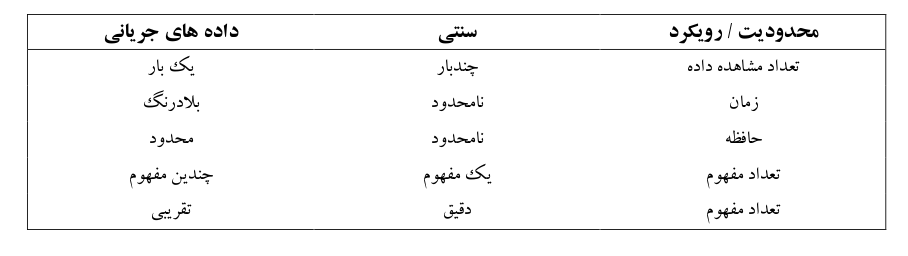
\includegraphics[width=\linewidth]{bound}
\end{table}


داده‌های جریانی با حجم نامتناهی، با اهمیت بودن ترتیب و زمان وقوع و تغییرات پویا شناخه می‌شوند. مثلا گوگل، میلیون‌های جستجو را روزانه پردازش می‌کند که هر کدامشان در یک زمان مشخص انجام شده‌اند و این جستجوها در طول زمان و براساس موضوعات داغ روز تغییر می‌کنند. جدول
\ref{tbl:bound}
تفاوت ویژگی‌های بین الگوریتم‌های داده‌های جریانی و الگوریتم‌های سنتی را نشان می‌دهد. به عبارت دیگر، اگر بخواهیم محدودیت‌های الگوریتم‌ها در فضای داده‌های جریانی را برشمریم باید از چهار محدودیت نام ببریم:


\begin{itemize}
\item یک‌بار مشاهده داده:\LTRfootnote{Single-pass } بر خلاف روش‌های یادگیری سنتی که می‌توانستند مجموعه‌‌ی داده را مکررا چند بار پیمایش کنند. الگوریتم‌ها در داده‌های جریانی فقط یک‌بار می‌توانند داده را مشاهده کنند و برگشت به عقبی وجود ندارد. دلیل این موضوع هم آن است که خواندن/نوشتن روی حافظه‌های جانبی بسیار هزینه‌بر تز از حافظه اصلی است. این محدودیت زیادی است و اگر به الگوریتم‌ها اجازه دهیم به جای یک داده چند داده را ببینند و اجازه داشته باشیند که چند نمونه به شکل کوتاه مدت ذخیره کنند اوضاع کمی بهتر می‌شود. به عنوان مثال یک الگوریتم می‌تواند یک دسته از نمونه‌ها را برای پردازش‌های داخلی ذخیره کند اما در نهایت باید با گرفتن یک دسته جدید از داده، داده‌های گذشته را پاک کند. 
\item پاسخ بلادرنگ:\LTRfootnote{Real-time Response} بسیاری از کاربردهای داده‌های جریانی نظیر پیش‌بینی بازار بورس، به پاسخ بلادرنگ نیاز دارند. میزان زمان مورد نیاز برای پردازش داده‌های و رسیدن به تصمیم باید کم باشد.
\item محدودیت حافظه: حجم‌ داده‌ای که می‌رسد خیلی بزرگ است و حتی ممکن است نامحدود باشد و ما می‌توانیم تنها تعداد کمی یا خلاصه‌ای از داده‌های جریانی را ذخیره‌ کنیم و ممکن است دیگر به اصل داده دسترسی نداشته باشیم. البته روش‌های تحمینی می‌توانند قابل قبول باشند.
\item تشخیص رانش‌ مفهوم: رانش‌ مفهوم زمانی است که الگوها(یا توزیع داده) در طی زمان تغییر پیدا می‌کند.
\end{itemize}

حال اگر منبع تولید جریان داده، منبعی باشد که متن تولید می‌کند مساله از جهاتی بغرنج‌تر می‌شود. پردازش و مدل‌کردن داده‌های متنی به دلیل غیر ساختیافته‌ بودن
\LTRfootnote{Unstructured}
، خطاهای سطح بالا
\LTRfootnote{High Level of Noise}
و وجود در فرمت‌های گوناگون بسیار پیچیده‌تر از سایر داده‌هاست. نفرین ابعاد
\LTRfootnote{Curse of Domensionality}
یکی از معضلات کار با داده‌های متنی است. در برخی از کاربردها، تعداد ویژگی‌هایی که از یک متن استخراج می‌شود چیزی بیش‌تر از دویست‌هزار ویژگی است. بنابراین لازم است که الگوریتم‌هایی در برابر داده‌های جریانی متنی به کار گرفته شوند که قابلیت سازگاری با این تعداد بسیار زیاد ویژگی را داشته باشند و یا این که با روش‌هایی نظیر پیش‌پردازش، انتخاب ویژگی و یا کاهش ابعاد، این داده‌ها را طوری به ورودی الگوریتم‌ها داد که محدودیت‌های زمانی و حافظه‌ای رعایت شود.
مضاف بر همه‌ی این مشکلات، در داده‌های متنی تعداد بسیار بیشتری از رویداد‌های تعجب‌آور و تغییر موضوعات شگفت‌انگیز مشاهده می‌شود. این موضوع باعث می‌شود که کاوش و یادگیری در داده‌های متنی یک وظیفه دلهره‌آور باشد. 








در این فصل به معرفی فضای کار در الگوریتم‌های یادگیری برای داده‌های جریانی پرداختیم، به علاوه مشکلات پیش‌رو زمانی که منبع داده‌ی ما یک منبع تولید کننده متن باشد را معرفی کردیم. در فصل‌ ۲ ابتدا به مرور ادبیات یادگیری در داده‌های جریانی خواهیم پرداخت و مفاهیمی نظیر منبع داده‌، مفهوم و رانش‌مفهوم را به شکل ریاضی تعریف می‌کنیم و سپس رویکردهای مختلف در برابر داده‌های جریانی را معرفی می‌کنیم. در این فصل علاوه بر ارایه تعاریف اولیه، مروری بر نرم‌افزارهای داده‌کاوی و یادگیری در فضای جریانی خواهیم داشت و مخزن‌های داده‌ی دردسترس را جهت تحقیقات و آزمایش‌های آتی معرفی خواهیم کرد. در فصل ۳ به معرفی الگوریتم‌های یادگیری ماشین در فضای داده های جریانی خواهیم پرداخت. این الگوریتم‌ها عموما نسخه‌های توسعه‌یافته از الگوریتم‌های سنتی یادگیری ماشین‌ هستند و با چالش‌ها و محدودیت‌های داده‌های جریانی سازگار شده‌اند. به طور کلی در این فصل الگوریتم‌هایی را معرفی خواهیم کرد که تغییر یافته الگوریتم‌های سنتی درخت تصمیم، یادگیرنده‌های بیز، شبکه‌های عصبی، ماشین‌های بردار پشتیبان و مجمع‌های رده‌بندی هستند. نهایتا در فصل ۴ و پایانی این گزارش، ابتدا به جمع‌بندی روش‌های یادگیری ارایه‌شده و مقایسه و نمایش نسبت الگوریتم‌ها با پدران سنتیشان می‌پردازیم سپس مزایا و معایب هر کدام را مطرح می‌کنیم و مشخص خواهیم کرد که کدام روش‌ها می‌توانند برای منابع جریانی داده‌های متنی به کار گرفته شوند. در نهایت نیز به جمع‌بندی کار و معرفی تحقیقات آینده،‌ نظیر انتخاب پویای ویژگی برای داده‌های جریانی خواهیم پرداخت.
			% فصل اول: مقدمه
% !TeX root=main.tex
% دستور زیر باید در اولین فصل شما باشد. آن را حذف نکنید!
\pagenumbering{arabic}

\chapter{مروری بر ادبیات}
\thispagestyle{empty}
\section{مقدمه}


\section{تعاریف اولیه}\label{sec2}
در این بخش به معرفی چند تعریف اولیه نظیر منبع داده، مفهوم، رانش مفهوم می‌پردازیم:
\subsection{جریان داده\LTRfootnote{Data Stream}}
یک جریان داده یه شکل یک دنباله از نمونه‌های داده تعریف می‌شود و آن را با نماد $DS$ نشان می‌دهیم:
$DS = \left\{ x_1, x_2, ..., x_t, ...\right\}$
که در این رابطه $x_i$ برابر i امین داده‌ی مشاهده شده است. هر نمونه داده‌ی $x_i$ یک برچسب دارد و با  $ y_i \in Y = \left\{y_1, y_2, ..., y_c\right\} $ نشان داده می شود.


\subsection{مفهوم\LTRfootnote{Concept}}
یک مفهوم یا یک منبع داده، توسط احتمال پیشین برای رده‌ها و تابع توزیع احتمال رده‌‌ی آن ها تعریف می شود:

\begin{equation}
S = \left\{(P(y_1), P(X|y_1));...;(P(y_c), P(X|y_c))\right\} 
\end{equation}
که در این رابطه y بیانگر رده‌ها است. روش‌های سنتی یادگیری ماشین و داده‌کاوی با یک مفهوم کار می‌کند، و این بدان معنی است که تابع توزیع احتمال مجموعه آموزش و مجموعه آزمون یکسان است. این در حالی است که داده‌های جریانی پویا هستند و تعداد زیادی مفهوم دارند. یک مثال از این تغییر مفهوم را می‌توانید حمله‌ی هکری در یک شبکه‌ی کامپیوتری را در نظر بگیرید. توضیح مفهوم داده‌ی «معمولی» با داده‌ی «حمله» در طی زمان تغییر می‌کند، همیشه حمله‌ها در حال انجام هستند ولی انواع و روش‌های آن تغییر می‌کند.
\\
یک جریان داده‌ای مانند DS شامل یک مجموعه k عضوی از منبع داده را در نظر بگیرید که در آن منابع داده با $s_i$ نشان‌ داده می‌شود و توزیع این منابع شناخته شده است $ i = 1, ..., k $. در زمان t یک یا چند منبع داده فعال وجود دارد. فرض کنید $w_i(t) \in [0, 1]$ برابر با تاثیر منبع داده  $S_i$ در زمان t باشد. توزیع داده‌ی جریان داده‌ی DS در زمان t توسط رابطه زیر مشخص می‌شود:

\begin{equation}
\sum^{DS}(t) = \left\{ w(1)S_1, ..., w(k)S_k \right\}
\end{equation}

\subsection{رانش مفهوم\LTRfootnote{Concept Drift}}

 اگر فرض کنیم که یک منبع داده DS شامل k منبع جریانی مستقل S با وزن اثر w باشند اگر در دو زمان $t_1$ و $t_2$ رابطه زیر برقرار باشد می گوییم رانش مفهوم رخ داده است.
\begin{equation}
\sum^{DS}(t_1) \neq \sum^{DS}(t_2)
\end{equation}
رانش‌های مفهوم به دو نوع زیر طبقه بندی می شوند:

\subsubsection{رانش مفهوم مجازی\LTRfootnote{Virtual Concept Drift}}
اگر رانش مفهوم تأثیر مستقیمی بر حدود تصمیم گیری نداشته باشد(احتمال پیشین داده ها تغییر نکند) اما رانش بر روی تابع چگالی احتمال اثر بگذارد گوییم که رانش مفهوم مجازی رخ داده است.

\subsubsection{رانش مفهوم حقیقی\LTRfootnote{Real Concept Drift}}
اگر رانش مفهوم علاوه بر تغییر تابع چگالی احتمال، تأثیر مستقیم بر حدود تصمیم گیری بگذارد و احتمال‌های پیشین را تغییر دهد گوییم رانش مفهوم حقیقی رخ داده است. روش های یادگیری در محیط‌های جریان‌های داده‌ای باید به گونه ای باشند که رانش مفهوم حقیقی سریعا تشخیص داده شود.

\section{پنجره‌های زمانی}
از آن‌جایی که داده‌های جریانی امکان دارد بینهایت باشند، تنها مقدور است که بخشی از تمام داده‌ی جریانی را پردازش شود. این بخش مورد توجه از داده توسط یک پنجره زمانی از نمونه‌های داده تعریف می‌شود.
\begin{equation}
W[i, j] = (x_i, x_{i+1}, ..., x_j)
\end{equation}
بر اساس این تعریف، انواع مختلفی از پنجره زمانی بیان‌ می‌شود: پنجره نقطه عطفی
\LTRfootnote{Landmark Window}
،پنجره کشویی
\LTRfootnote{Sliding Window}
،پنجره محو شونده
\LTRfootnote{Fading Window}
و پنجره یک‌بر
\LTRfootnote{Tilted Window}.

\subsection{پنجره نقطه عطفی}
در پنجره نقطه عطقی، ما به تمام داده جریانی از زمان شروع نمونه اول تا زمان فعلی نمونه $ t_c $ توجه می‌کنیم: پنجره به شکل $ W[1, c] $ تعریف می‌شود. استفاده از این پنجره نقطه عطفی بدین معناست که تمامی تراکنش‌ها در پنجره به شکل یکسانی برای ما اهمیت دارند، هیچ تفاوتی داده‌های گذشته و حال وجود ندارد. به طور مداوم که داده‌های جریانی تغییر می‌کنند، مدل با استفاده از داده قدیمی نمونه‌ها ساخته می‌شود که حتی ممکن است که با داده‌های جدید ناسازگار باشند. برای تاکید بیشتر روی داده‌های جدیدتر می‌توان از پنجره‌های کشویی، محوشونده و یک بر استفاده کرد.
\subsection{پنجره کشویی}
   در پنجره کشویی که با
$W[t_c - w + 1, t_c]$
 نشان داده می‌شود ما تنها به w تراکنش اخیر توجه می‌کنیم و بقیه داده‌های جریانی نادیده گرفته‌ می‌شوند. نتیجه کاوش وابسته به اندازه پنجره است که w بیانگر آن است. اگر w خیلی بزرگ باشد و رانش مفهوم رخ دهد، پنحره ممکن است شامل داده‌‌ها و اطلاعات منقضی شده باشد و دقت مدل کاهش پیدا می‌کند. اگر w کوچک باشد، پنجره ممکن است شامل داده‌های ناکار باشد و مدل دچار بیش‌برازش گردد.
کارهای قبلی یک مقدار ثابت را برای اندازه پنجره کشویی در نظر‌ می‌گرفتند که توسط کاربران و با آزمایش تعیین می‌شد. اخیرا چند کار برای ارایه پنجره کشویی انعطاف پذیر ارایه شده است که در آن اندازه پنجره بر اساس دقت مدل تغییر می‌کند. زمانی که دقت زیاد باشد اندازه پنجره بزرگ می‌شود و زمانی هم که دقت کم شود، پنجره کوچک می‌شود.

\subsection{پنجره محوشونده}
در پنجره‌های محو شونده، هر نمونه از داده‌های جریانی به یک وزن که با زمان رسیدن آن نمونه در ارتباط است شناسایی می‌شود، بنابراین داده‌های جدیدتر می‌رسند وزن بیشتری از داده‌های قدیمی‌تر دارند. با استفاده از پنجره محو شونده، می‌توان تاثیر(اهمیت) داده‌های قدیمی منقرض شده را کاهش داد تا در نتیجه کاوش تاثیری نداشته باشند. معمولا از یک تابع نمایی نزولی مانند تابع زیر برای پنجره زمانی استفاده می‌شود:
\begin{equation}
f(\triangle t) = \lambda^{\triangle t}(0 < \lambda < 1)
\end{equation}
در این تابع $\triangle t$ قدمت(سن) نمونه داده‌ی جریانی و برابر با تفاوت زمانی فعلی و زمان مشاهده داده است. پنجره محو شونده نیاز به انتخاب یک پارامتر محوشوندگی مانند $ \lambda $ دارد که معمولا یک عدد در بازه $ [0.99, 1] $ برای کاربردهای واقعی انتخاب می‌شود.

\subsection{پنجره یک‌بر}
پنجره یک‌بر یک نوع پنجره زمانی شبیه پنجره محو شونده و کشویی است. این پنجره در سطوح مختلف ریزدانگی که با توجه به تاخر داده شکل گرفته‌اند اعمال می‌شود. پنجره زمانی‌ یک‌بر تقریبا تمام مجموعه داده را ذخیره کرده و یک تعادل بین فضای مورد نیاز برای ذخیره‌سازی و دقت برقرار می‌کند. البته این‌ مدل می‌تواند پس از اجرای طولانی غیر پایدار باشد.

\begin{figure}%[ht]
\centerline{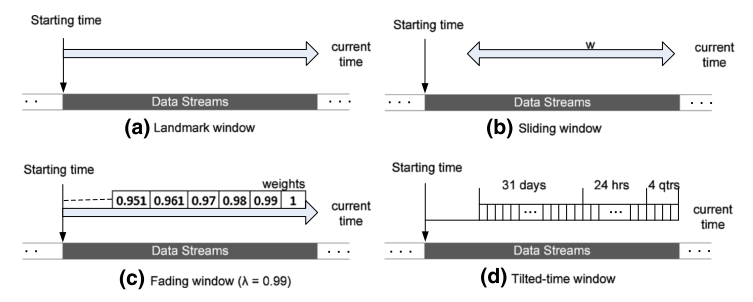
\includegraphics[width=15cm]{time-windows}}
\caption{پنجره‌های مختلف زمانی}
\label{fig:time-windows}
\end{figure}
تصویر
\ref{fig:time-windows}
چهار نوع مختلف پنجره زمانی را نشان می‌دهد. برای پنجره محو شونده $\lambda$ برابر با $0.99$ تنظیم شده است و وزن نمونه‌ها کاهش می‌یابد. برای پنجره یک‌بر، ما جهار ربع اخیر یک ساعت را ذخیره کرده‌ایم، سپس ۲۴ ساعت گذشته و ۳۱ روز اخیر نمایش داده شده‌اند.




\section{رویکردهای محاسباتی}

براساس انواع مختلف پنجره زمانی، دو رویکرد محاسبانی مختلف برای پردازش داده‌های جریانی وجود دارد.

\subsection{یادگیری افزایشی\LTRfootnote{Incremental Learning}}
یادگیری افزایشی یک رویکرد محاسباتی برای داده‌های جریانی است. در این رویکرد، مدل به صورت افزایشی تغییری می‌کند تا با تغییرات در داده‌هایی که در حال آمدن هستند، سازگار شوند. دو طرح کلی برای بروزرسانی مدل وجود دارد: بروزرسانی با هر نمونه داده و بروزرسانی با پنجره. به عنوان نمونه ستریت
\LTRfootnote{Street}
و همکارانش یک مجمع از رده‌بندها برای داده‌های جریانی توسعه‌ دادند که این مجمع یک پنجره از داده‌های ورودی را می‌گیرد و مدل را با تنظیم وزن‌های هر رده‌بند یا جایگزین کردن رده‌بند‌های قدیمی با نمونه‌های جدیدشان سازگار می‌کند. شکل
\ref{fig:approach}
- الف رویکرد یادگیری افزایشی را نمایش می‌دهد. مزیت این رویکرد این است که نتیجه برای هر نمونه(یا پنجره‌ای از نمونه‌ها) در دسترس است ولی به منبع محاسباتی بیشتری نیاز است.
\subsection{یادگیری دوگامی\LTRfootnote{Two-Phase Learning}}
یادگیری دوگامی، که با نام یادگیری آنلاین-آفلاین نیز شناخته می‌شود یک رویکرد محاسباتی برای داده‌های جریانی است. ایده‌ بنیادی این است که کاوش بر داده‌ها را به دو بخش تقسیم کنیم. در گام اول(گام آنلاین)، چکیده‌ای از داده در لحظه ایجاد می‌شود. در گام دوم(گام آفلاین)، بر مبنای درخواست کاربر، پردازش روی چکیده‌هایی کع در گام قبل ایجاد شده بود انجام می‌شود.
به عنوان مثال، آگراول
\LTRfootnote{Aggarwal}
 و همکارانش، یک روش آنلاین-آفلاین برای خوشه‌بندی داده‌های جریانی ارایه کرده‌اند که در بخش آنلاین، خلاصه‌ای از اطلاعات آماری داده جریانی به صورت برخط گردآوری می‌شود. در طول بخش آفلاین، از این داده‌ها برای خوشه بندی سطح بالا استفاده می‌شود. رویکرد یادگیری دوگامی در شکل نشان داده شده است. این روش قابلیت پردازش داده های جریانی را با سرعت بیشتری داد منتها محدودیت آن این است که کاربر باید تا فراهم شدن نتیجه، منتظر بماند.
شکل
\ref{fig:approach}
- ب رویکرد یادگیری آنلاین-آفلاین را نمایش می‌دهد.




\begin{figure}%[ht]
\centerline{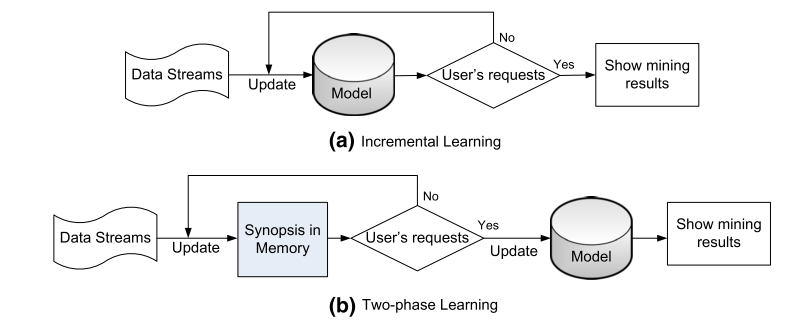
\includegraphics[width=15cm]{approach}}
\caption{الف- رویکرد افزایشی به یادگیری. ب- رویکرد دو گامی}
\label{fig:approach}
\end{figure}


\section{اعتبار سنجی}
در روش‌های سنتی یادگیری ماشین با مقدار داده‌ی محدود، فرآیند اعتبارسنجی بر استفاده‌ی بیشینه از داده تمرکز داشت. جداسازی
\LTRfootnote{Hold-out}
اعتبار سنجی متقابل
\LTRfootnote{Cross-Validation}
، تک‌گذاری
\LTRfootnote{Leave-One-Out}
روش‌های استاندارد اعتبار سنجی هستند. در روش جداسازی به شکل تصادفی مجموعه‌ی داده به دو زیر مجموعه، یکی برای آموزش و دیگری برای آزمایش تقسیم می‌شود. نسبت‌های رایج برای تقسیم داده به مجموعه آموزش و آزمایش نصف و یک‌سوم است. در روش اعتبار سنجی متقابل با k دسته، داده به k مجموعه‌ی مساوی و مستقل از نمونه‌ها تقسیم می‌شد و یکی از این زیر مجوعه‌ها برای آزمایش و باقی آن‌ها( $k-1$ )برای آموزش ادغام می‌شد. در این روش فرآیند اعتبار سنجی k بار و هر بار با یک زیر مجموعه برای آزمایش انجام می‌شود. روش تک‌گذاری نیز یک نوع اعتبار سنجی متقابل است که در آن k با تعداد کل داده‌ها برابر است.
\\
در محیط جریان‌های داده‌ای، از آن‌جایی که داده می‌تواند نامحدود باشد، اعتبار سنجی بر ارزیابی مدل در صحنه‌های مختلف متمرکز است. یک روش شناخته‌شده رسم منحنی یادگیری با ذخیره‌سازی کارایی مدل در طول زمان است. این منحنی نشان‌ خواهد داد که چقدر مدل پس از مشاهده‌ی داده‌های بیشتر، بهتر شده است و مدل چگونه با رانش‌ مفهوم سازگار می‌شود. یک الگوریتم برتری خود را به سایر روش‌ها زمانی نشان می‌‌دهد که منحنی یادگیریش بیشتر مواقع از سایر الگوریتم‌ها بالا‌تر باشد.
\\
روش جداسازی و روش پی‌درپی
\LTRfootnote{Prequential}
دو روش پر کاربرد برای اعتبارسنجی جریان‌های داده‌ای هستند. در روش جداسازی، نمونه‌های داده به چانک‌های مختلفی تقسیم می‌شوند. از هر چانک داده ابتدا برای آزمایش و سپس برای بروزرسانی مدل استفاده می شود. روش جداسازی زمانی که رانش‌ مفهوم رخ داده، ترجیح داده می‌شود چون این روش اجازه می‌دهد که مدل با آخرین تغییرات داده سازگار شود. روش پی‌در‌پی(یا آزمایش-سپس-آموزش
\LTRfootnote{Test-Then-Train}
به شکل لایه‌ لایه) یک روش دیگر برای ارزیابی جریان‌های داده‌ای است. هر نمونه داده ابتدا و پیش از این‌که برای آموزش به صورت افزایشی استفاده شود، برای آزمایش استفاده می‌شود. این روش می‌تواند یک حالت خاص برای روش جداسازی در نظر گرفته شود اگر اندازه چانک برابر با یک باشد. مزیت این روش این است که نیازی به تعریف از پیش اندازه چانک نیست ولی متاسفانه کارایی این الگوریتم در زمان محدود  مبهم است چراکه اشتباهات اولیه مدل به سرعت در طول زمان کاهش می‌یابد.


\subsubsection{معیارهای ارزیابی}


به طور عمومی معیارهای ارزیابی روش‌های سنتی یادگیری ماشین، می‌تواند برای ارزیابی یادگیرنده‌ها در جریان‌های داده نیز استفاده شود. برای رده‌بندی داده‌ها، صحت
\LTRfootnote{Accuracy}
و تابع ضرر $0-1$ دو معیار رایج هستند. برای ارزیابی مداوم کارایی رده‌بندی در داده‌های جریانی، گیم
\LTRfootnote{Game}
و همکارانش یک روش ضرر پی‌در‌پی که با انواع مختلف پنجره کار می‌کند را ارایه کرده‌اند. برای از یاد‌بردن پی‌در‌پی خطا اثبات شده است که همگرایی خطای بیز در داده‌های ایستا، روش را برای تشخیص رانش کارا می‌سازد. این روش می‌تواند به سادگی روی سایر معیار‌های کارایی نیز اعمال شود.

\section{نرم‌افزارهای کاربردی}
نرم‌افزارهای مختلف کاربری و متن‌باز برای تحقیقات دانشگاهی در حوزه‌ی یادگیری و داده‌کاوی در محیط‌های پویای جریان‌های داده‌ای وجود دارد.

\subsubsection{WEKA}
شناخته‌شده‌ترین ابزار داده‌کاوری در محیط دانشگاهی است. این ابزار شامل یک مجوعه از الگوریتم‌های پردازی داده، رده‌بندی، رگرسیون، خوشه‌بندی، قواعد باهم‌آیی و بصری سازی داده است.

\subsubsection{MOA}
نرم افزار MOA یک فریمورک متن‌باز محبوب برای داده کاوی در داده های جریانی است که توسط دانشگاه وایکیتو نیوزلند
\LTRfootnote{University of Waikato, New Zealand}
 و بر مبنای چهارچوب  WEKA توسعه داده شده است. در این نرم افزار که توسط زبان جاوا پیاده سازی شده، تعداد زیادی ابزار مناسب جهت پیاده سازی و تست الگوریتم های یادگیری و خوشه بندی و تشخیص رانش مفهوم وجود دارد. برای نمونه الگوریتم‌های درخت‌ تصمیم خیلی سریع و مجمع رده‌بند ها که در ادامه توضیح داده‌ می‌شوند در این چهارچوب موجود است.
این ابزار تعدادی تولید‌‌کننده
\LTRfootnote{Generator}
 داده جریانی مانند مفهوم‌های SEA  ،ابرصفحه‌ی دوران کننده
\LTRfootnote{Rotating Hyperplane}
 و STAGGER را فراهم کرده است.
\subsubsection{Rapid-Miner}

یکی دیگر از ابزارهای متن‌باز برای داده‌کاوی است. RapidMiner بسیار قدرتمندتر از WEKA است و تمام الگوریتم‌های WEKA و سایر الگوریتم‌های پیشرفته را دارد. این ابزار خلاقانه‌تر است و این قابلیت را داد که پروسه داده‌کاوی را به شکل یک دنباله از عملگرها تعریف کرد. همچنین RapidMiner ابزارهای بیشتری را بصری‌سازی فراهم کرده است.
\section{مخزن‌های داده}
داده‌های واقعی بسیار کمی برای ارزیابی روش‌های یادگیری در داده‌های جریانی وجود دارد. یک دلیل این ‌موضوع می‌تواند این باشد که محققان روش‌های سنتی داده‌کاوی و یادگیری ماشین معمولا داده‌های خود را به قدری کوچک نگه‌می‌داشتند تا با روش‌های یادگیری دسته‌ای
\LTRfootnote{Batch Learning}
سازگار باشد.
\\
 یک دلیل دیگر می‌تواند مساله حریم شخصی در انتشار داده‌های که خیلی بزرگ هستند باشد. محققان معمولا از داده‌های خصوصی برای اثبات سیستم‌هایشان استفاده می‌کنند که نمی‌توانند آن‌ها را منتشر کنند. برای غلبه بر این کمبود، بعضی از مجموعه داده‌های ترکیب شده با تعداد نامحدود داده ساخته شده‌اند. برای مثلا تولید کننده ‌درخت تصادفی، تولید‌ کننده مفهوم SEA و ابرصفحه‌های چرخنده تولید شده‌اند. این تولیدکننده‌های داده در چهارچوب MOA پیاده‌سازی شده‌اند. بعضی از مخزن‌های داده با مجموعه‌های داده‌ی بزرگ نیز برای ارزیابی روش‌های یادگیری در داده‌های جریانی استفاده می شود:
\subsubsection{\lr{UCI Machine Learning Repository\LTRfootnote{http://www.ics.uci.edu/~mlearn/mlrepository.html}}}
یک مخزن آنلاین معتبر  و شناخته شده برای آزمایش و آنالیز الگوریتم‌های یادگیری ماشین است. سه مجموعه داده پر استفاده در چندین مقاله برای ارزیابی جریان‌ها Forest Covertype و Poker-Hand و Electricity هستند.
\subsubsection{\lr{KDD Cup Center}}
رقابت‌های سالانه‌ی داده‌کاوی و کاوش دانش توسط
\lr{ACM Special Interest Group\LTRfootnote{http://www.kdd.org/}}
سازمان‌دهی می‌شود. معمولا داده‌هایی که برای این رقابت تولید می‌شود می‌تواند منبع خوبی برای ارزیابی الگوریتم‌های یادگیری ماشین در داده‌های جریانی باشد.
		% فصل دوم: آشنایی مقدماتی با لاتک
% !TeX root=main.tex
% دستور زیر باید در اولین فصل شما باشد. آن را حذف نکنید!

\chapter{روش‌های یادگیری در داده‌های جریانی}
\thispagestyle{empty}
رده‌بندی فرایند یافتن یک مدل عمومی از داده‌های گذشته است به طوری که بتوان آن مدل را روی داده‌های جدید اعمال کرد. رده‌بندی از دو گام تشکیل شده است: گام یادگیری(آموزش) و گام تست. در بخش یادگیری سیستم تلاش می‌کند که یک مدل از مجموعه‌ی داده‌های نمونه‌ی مجموعه آموزشی یاد بگیرد؛ در گام تست از این مدل برای برچسب‌زنی به داده‌هایی که برچسب زده‌نشده‌اند استفاده می‌شود. در ادبیات داده‌های جریانی، تعداد زیادی الگوریتم رده‌بندی مانند درخت‌های تصمیم، رده‌بند بیزین، ماشین‌های بردار پشتیبان، k نزدیک‌ترین همسایگی و روش‌هایی که مجمعی از رده‌بندها را می‌سازند وجود دارد. در این فصل به بررسی این روش‌ها می‌پردازیم و روش کار هر کدام را به شکل مختصر توضیح می‌دهیم.

\section{درخت هافدین}\label{sec3}
درخت هافدین یک رده‌بند بر مبنای درخت تصمیم برای داده‌های جریانی است\cite{gama2007learning}. روش‌های سنتی درخت تصمیم، برای انتخاب خصیصه تقسیم نیاز به چندین بار پویش داده دارند که این موضوع در محیط داده‌های جریانی، عملا نشدنی است. سایر روش‌های رده‌بندی داده‌های جریانی نیز معمولا کاستی‌هایی مانند موارد زیر دارند:


\begin{itemize}
\item حساسیت زیاد به ترتیب نمونه‌ها
\item کارایی کم. در بعضی موارد آن‌های از الگوریتم‌های یادگیری دسته‌ای کندترند.
\end{itemize}
درخت هافدین که یکی از روش‌های جدید یادگیری برای جریان‌هاست چالش‌های زیر را حل می‌کند:

\begin{itemize}
\item عدم قطعیت در زمان یادگیری. زمان یادگیری در درخت هافدین برای هر نمونه ثابت است و این بدان معنیست که درخت هافدین برای کاوش در داده‌های جریانی مناسب است.
\item زمانی که تعداد نمونه کافی برای ساخت درخت پویش شود، نتیجه درخت‌ در روش هافدین تقریبا مشابه(یا برابر) با درخت‌های ساخته شده با روش‌های مرسوم یادگیری دسته‌ای است.
\end{itemize}

برای تعامل با چالش پویش چندباره داده‌ها از حد هافدین برای انتخاب یک خصیصه تقسیم بهینه، پس پویش تعداد کافی نمونه استفاده می‌شود. فرض کنید N تعداد مشاهدات مستقل از یک متغییر تصادفی r باشد که این متغییر تصادفی در محدود R و با میانگین $ \overline{r} $ است. حد هافدین تضمین می کند که میانگین درست r حداقل از $ \overline{r} -\epsilon $ با احتمال $ 1 - \delta $ بزرگ‌تر باشد. در این رابطه $ \delta $ پارامتری است که کاربر انتخاب می‌کند.

$$ P(E[r] \geq (\overline{r} - \epsilon)) \geq 1 - \delta, \epsilon = \sqrt{\frac{R^2ln(\frac{1}{\delta})}{2N}} $$


چیزی که حد هافدین را جالب توجه می‌کند، امکان گرفتن نتیجه‌های مشابه بدون در نظر گرفتن توزیع احتمالی‌ست که مشاهدات را تولید می‌کند. به عنوان نمونه اگر اختلاف بهره اطلاعاتی بین دو خصیصه A و B (که می‌دانیم بهره اطلاعاتی خصیصه A بیشتر از خصیصه B است) برابر با $0.3$ و $ e=0.1 $ باشد این معنی را می‌دهد که در آینده، تفاوت بین بهره اطلاعاتی A و B حداقل $ 0.3 - 0.1 = 0.2 $ است. به عبارت دیگر با احتمال $1 - \delta$، هنگامی که تفاوت بهره اطلاعاتی مشاهده شده بزرگ‌تر از  $ \epsilon $ باشد یک خصیصه در مقایسه با دیگر خصیصه‌ها قالب است.

فرض کنیم $ G(x_{i}) $ یک معیار اکتشافی برای انتخاب کردن خصیصه جداسازی باشد و پس از مشاهده N نمونه، $x_{a}$ و $x_{b}$ اولین و دومین خصیصه برتر برای خصیصه جداسازی باشند. با این مفروضات، در درخت هافدین، متغییر r از رابطه $ r = \triangle G = G(X_a) - G(X_b) $ تعیین می‌شود.
 اگر $ \overline{r} = \triangle \overline{G} = \overline{G}(X_a) - \overline{G}(X_b) $ باشد که در آن $\epsilon $ از رابطه بالا محاسبه شده است،
می‌گوییم با اطمینان $1 - \delta $ این تفاوت بزرگتر از $ \overline{r} - \epsilon > 0 $ است. بنابراین خصیصه $x_{a}$ برای جداسازی انتخاب می‌شود.


نویسندگان الگوریتم درخت هافدین را توسط یک یادگیرنده با نام «درخت تصمیم خیلی سریع»(VFDT) پیاده‌سازی کرده‌اند. این پیاده‌سازی شامل بهبودهایی برای استفاده‌های خاص، مانند راهبرد محدود کردن گره، راهندازی سریع با استفاده از یادگیرنده‌های مبتنی بر RAM و قابلیت بازپویش نمونه‌های قبلی زمانی که سرعت گذر داده کم است می‌باشد.
\\
الگوریتم درخت هافدین،‌ یک الگوریتم با دقت بالاست که می‌تواند بسیار خوب با مجموعه‌ی داده‌های بزرگ کار کند، ولی این الگوریتم نمی‌تواند با مساله رانش مفهوم در داده‌های جریانی تعامل کند\cite{Nguyen2015}. الگوریتم CVFDT \cite{hulten2001mining} یک تعمیم از الگوریتم درخت هافدین است که برای تعامل با رانش مفهوم در داده‌های جریانی  سازگار شده است. CVFDT ، بعضی آماره‌های کارآمد را برای بررسی کردن اعتبار تصمیم‌های قبلی در کنار هر گره درخت نگهداری می‌کند. زمانی که یک داده وارد می‌شود، به طور مداوم این آماره‌های قرارگرفته در کنار گره‌های درخت بروزرسانی می‌شوند. با کمک پنجره‌های جابه‌جا شونده روی داده، این الگوریتم اثر داده‌هایی که از پنجره خارج هستند را در آماره‌های هر گره نادیده می‌گیرد. این پویش دوره‌ای گره‌های درخت‌ باعث تشخیص رانش مفهوم می‌شوند. اگر رانش مفهوم ظاهر شده باشد، CVFDT یه صورت موازی شاخه‌های جایگزین را با انتخاب بهترین خصیصه‌های جدید و حذف شاخته‌های قدیمی، اگر دقتشان کم باشد، گسترش می‌دهد.

\section{رده‌بند بیزین}

سیدل
\LTRfootnote{Seidl}
و همکارانش \cite{seidl2009indexing} یک روش جالب برپایه نمایه‌سازی
\LTRfootnote{Index-Based}
رده‌بند ارایه داده‌اند که درخت بیز نامیده می‌شود. درخت بیز از یک درخت مخلوط-گوسین سلسله مراتبی
\LTRfootnote{Hierarchical Gaussian-mixture Tree}
جهت نمایان‌کردن تمام مجموعه‌ی داده استفاده می‌کند. هر گره از درخت شامل آماره‌های از نمونه‌های داده مثل مستطیل محدود‌کننده کمینه
\LTRfootnote{Minimum Bounding Rectangle}
، تعداد نمونه‌های داده، جمع خطی و مجموع مربعات تمام داده است.
برای حل مساله‌ی رده‌بندی چند کلاسه، یک درخت بیز برای هر کلاس ساخته‌ می‌شود.برای هر داده‌ی ست مانند x    ، الگوریتم سعی می‌کند که نزدیک‌ترین مجموعه گره‌ها را که مرز نامیده می‌شوند پیدا کند. احتمال تعلق x به کلاس $c_i$ توسط رابطه زیر محاسبه می‌شود:

$$
P(c_i | x ) = 
\left(       
\sum_{e_s \in E_i} \frac{n_{e_s}}{n}
g(x, \mu_{e_s}, \sigma_{e_s})
\right)
\star P(c_i)/P(x)
$$


که در این رابطه $e_s$ یک گره درخت در مخموعه مرز $E_i$ است. $n_{e_s}$ و $ \mu_{e_s}$ و $\sigma_{e_s}$ به ترتیب، تعداد نمونه‌های داده،‌مرکز و انحراف گره $e_s$ هستند. برای مشخص کردن برچسب نمونه‌ی x ، احتمال برای تمام کلاس‌ها حساب می‌شود و کلاسی که بیشترین احتمال را داشته‌باشد به عنوان کلاس نمونه x اعلام می‌شود. درخت بیز یک رده‌بند است که پس از مدت کمی از شروع، می‌تواند نتیجه و تصمیم داشته باشد و سپس آن دقت‌ها را با انتخاب مرز‌های دقیق‌تر افزایش دهد.


\section{شبکه عصبی}
لیت
\LTRfootnote{Leite}
و همکارانش \cite{leite2010evolving} روش شبکه‌های عصبی داده‌دانه تغییر پذیر
\LTRfootnote{Evolving Granular Neural Network}
(eGNN)
را جهت رده‌بندی داده‌های جریانی ارایه داده‌اند. دو گام در eGNN وجود دارد؛ در گام اول، eGNN از نرون‌های T-S برای ساختن ریزدانه‌های اطلاعات برای داده‌هایی که درحال آمدن هستند، استفاده می‌کند؛ در گام دوم، شبکه عصبی روی این ریزدانه‌های اطلاعاتی، به جای داده‌ی اصلی، ساخته می‌شود. یک ریزدانه مرتبط با برچسب یک کلاس به شکل یک تابع عضویت سه‌گوش
\LTRfootnote{Triangular membership function}
 تعریف می شود که بعدا جهت تطبیق با داده‌های جدید تغییر می‌کند.
 
  وزن‌ها با یک ثابت زوال
\LTRfootnote{Decay}
کاهش پیدا می‌کنند؛ این پردازش کمک می‌کند که درجه اهمیت ریزدانه‌های منقضی شده کاهش پیدا کند. به شکل پایه، eGNN از نمونه‌های کلاس در فرم ریزدانه‌های اطلاعاتی جهت انجام رده‌بندی استفاده می‌کند. زمانی که داده‌های تست می‌آیند یک نرون بیشینه‌گیری، بهترین پیش‌بینی ریزدانگی را انتخاب می‌کند و برچسب آن را به نمونه، جهت پیشبینی کلاسش، اختصاص می‌دهد. eGNN می‌تواند در مساله رده‌بندی در محیط‌های که دایما تغییر می‌کند استفاده شود اما نیاز به زمان طولانی آموزش، هنوز یک محدودیت برای شبکه‌های eGNN به منظور کار با داده‌های بسیار بزرگ است. البته، در قسمت آزمایش‌های مقاله اصلی، مجموعه‌های داده‌ی کوچک برای ارزیابی این روش استفاده شده است؛ سپس نویسنده، این روش‌ را جهت کارایی بهتر و کار به شکل نیمه نظارتی \LTRfootnote{Semi-Supervised} گسترش داده‌است تا با مجموعه‌ی داده‌هایی که کاملا برچسب گذاری نشده‌اند هم کار کند. 

\section{ماشین‌های بردار پشتیبان}
ماشین‌های بردار پشتیبان
\LTRfootnote{Support Vector Machine}
کارایی خود را در بسیاری از مساله‌های یادگیری ماشین با داده‌های ایستا نشان داده‌‌اند\cite{Nguyen2015}. البته استفاده از ماشین‌های بردار پشتیبان برای کاربردهایی با مقیاس بزرگ بسیار پرهزینه است. اگر N تعداد نمونه‌های داده باشد، این الگوریتم از پیچیدگی زمانی $ O(N^3) $ و از پیچیدگی حافظه‌ای $ O(N^2) $ است. برای کار کردن با داده‌های بسیار بزرگ، تی‌سنگ
\LTRfootnote{Tsang}
و همکارانش، الگوریتم ماشین بردار هسته
\LTRfootnote{Core Vector Machine}
(CVM)
 را ارایه داده‌اند تا پیچیدگی الگوریتم ماشین بردار پشتیبان را کاهش دهند. این الگوریتم از حداقل گوی نزدیک(MEB) برای این کار استفاده می‌کند. یک MEB ابر کره
\LTRfootnote{Hypersphere}
(کره با بیش از سه بعد) است که نماینده یک مجموعه از نمونه‌های داده کنار آن است\cite{tsang2007simpler} . این الگوریتم ابتدا MEB های نماینده را که تخمین خوبی از داده اصلی باشند، پیدا می‌کند. سپس مساله بهینه‌سازی پیدا کردن محدوده‌ی بیشینه بر روی این مجموعه‌های MEB اعمال می‌شود.


ری
\LTRfootnote{Rai}
و همکارانش  \cite{rai2009streamed} الگوریتم دیگری با نام StreamSVM که یک بهبود از الگوریتم CVM است را برای کار با داده‌های جریانی ارایه کرده‌اند. در این الگوریتم، یک MEB شعاع انعطاف پذیری است، هرزمان نمونه‌های جدید آموزش اضافه می‌شوند، این شعاع افزایش می‌یابد. این الگوریتم زمانی که تخمین‌ها درست باشند با بهینه‌ترین روش‌ها قابل رقابت است، اما StreamSVM هنوز قابلیت تشخیص رانش‌ مفهوم در داده‌های جریانی را ندارد.


\section{رده‌بند نزدیک‌ترین همسایگی}

در مورد خوشه بندی جریان‌های داده‌ای(که مورد بحث این گزارش نیست)، یک روش خوشه‌بندی با نام CluStream وجود دارد. این روش از تعریفی تحت عنوان ریز-خوشه
\LTRfootnote{Micro-Cluster}
برای خوشه‌بندی داده‌ها استفاده می‌کند. یک ریز-خوشه برای تعدادی داده، شامل آماره‌هایی نظیر مجموع مربعات نقاط، مجموع نقاط، مجموع مربعات زمان رخداد نقاط، مجموع خطی زمان رخداد و تعدا نمونه‌هاست. این روش خوشه‌بندی به جای ذخیره کل داده‌های خوشه، در گام آنلاین ریز-خوشه‌های آن‌ها که حجم کمتری را اشغال می‌کند و پردازش آن آسان‌تر است را ساخته و ذخیره می‌کند و در گام آفلاین به جای خوشه‌بندی کل داده‌ها، این ریز-خوشه‌ها را خوشه‌بندی می‌کند\cite{Nguyen2015}.
روش On-Demand-Stream \cite{aggarwal2003framework} یک گسترش از روش CluStream است که همانند این روش، از رویکرد آنلاین-آفلاین و پنجره یک‌بر استفاده می‌کند. تفاوت ریز-خوشه در این روش با ریز-خوشه در روش CluStream این است که برچسب کلاس نیز به ریز-خوشه اضافه می‌شود و ریز-خوشه‌ها فقط شامل نمونه‌هایی از یک کلاس مشخص و یکسان هستند. در رده‌بندی آفلاین، سعی می‌شود که بهترین پنجره از نمونه‌های داده که افق زمان
\LTRfootnote{Time Horizon}
نامیده می‌شود انتخاب شود و ریز-خوشه‌ها از این افق زمانی استخراج می‌شوند. روش On-Demand-Stream از یک رده‌بندی 1NN برای نسبت‌دادن داده‌ی آزمایش به نزدیک‌ترین ریز-خوشه استفاده‌ می‌کند.

با الهام‌گرفتن از ایده M-tree، ژنگ و همکارانش  \cite{zhang2011enabling} یک روش ساختار Lazy-tree برای نمایه سازی ریز-خوشه‌ها پیشنهاد داده‌اند. این کمک می‌کند که پیچیدگی زمانی روش‌ نزدیک‌ترین همسایگی اگر فرض کنیم N تعداد ریز-خوشه‌ها در Lazy-tree باشد، از $O(N)$ به $ O(log(N))$ کاهش یابد. درخت شامل سه عملگر اصلی است: جستجو، حذف و افزودن. اضافه‌کردن و حذف‌کردن برای افزودن گره‌های جدید و حذف‌کردن گره‌های منقضی شده به کار‌ می‌رود و تضمین می‌کنند که درخت متعادل بماند. عملگر جستجو برای رده‌بندی داده‌های تست استفاده می‌شود.


\section{مجمع رده‌بندها}
روش‌های
\lr{Bagging $ \& $ Boosting}
برتری خود را از طریق آزمایش‌ها روی مجموعه‌ی داده‌های سنتی اثبات کرده‌ است، نظر به این موضوع، بسیاری از محققین تلاش کرده‌اند که این روش‌ها را برای کار روی داده‌های جریانی سازگار کنند.
اوزا
\LTRfootnote{Oza}
و همکارانش \cite{oza2005online} روشی تحت عنوان
\lr{Bagging $ \& $ Boosting}
آنلاین ارایه کرده‌اند که یکی از اولین‌ کار‌ها برای سازگار کردن این روش بوده است. با دید آماری، هر نمونه از داده‌های آموزشی k بار در مجموعه‌‌ی آموزشی اعضای رده‌بند با احتمال زیر مشاهده می‌شود:

$$
P(k) = \left(\begin{array}{c}N\\ k\end{array}\right)
\left(\frac{1}{N} \right)^{k}
\left(1 - \frac{1}{N} \right)^{N-k}
$$
که در رابطه k اندازه مجموعه‌ی آموزشی و N اندازه مجموعه‌ی داده‌هاست. در داده‌های جریانی می‌توان فرض کرد که تعداد نمونه‌های داده نامحدود است، لذا $N \rightarrow \infty$؛ بنابراین احتمال $ P(k) $ به توزیع احتمال پوآسون میل می‌کند که رابطه آن مشابه زیر است:
$$Poisson(1) = exp(−1)/k!$$
با این مشاهده، اوزا و همکاران روش
\lr{Online Bagging}
را جهت نسبت دادن هر شی از داده به یک وزن متناسب با توزیع پواسون ارایه کردند. در
\lr{Online Boosting} 
وزن‌های داده‌هایی که در حال آمدن هستند و اعضای رده‌بندها بر اساس نسبت خطای اعضای رده‌بند به خطای کنونی تنظیم می‌شود.
\subsection{مجمع وزنی رده‌بند‌ها}
نظر به منقضی شدن داده‌های قدیمی، باید به توزیع داده به جای زمان رسیدن داده اعتماد کرد. بر این اساس ونگ
\LTRfootnote{Wang}
و همکارانش \cite{wang2003mining} یک روش دقت-وزن‌ برای مجمع رده‌بندها
\LTRfootnote{Accuracy-Weighted Ensemble}
(AWE)
ارایه کردند تا بتوان رانش مفهوم را در داده‌های جریانی کاوش کرد. الگوریتم با تعداد k رده‌بند که می‌توانند $RIPPER$ یا $C4.5$ یا بیزین ساده باشند ایجاد می‌شود و با همان تعداد نیز نگهداری می‌شود. با استفاده از یک تکه از نمونه‌های داده‌ای که در حال آمدن هستند یک رده‌بند جدید آموزش داده می‌شود؛ سپس مجمع با انتخاب k امین رده‌بندهای با دقت سازمان‌دهی می‌شود و وزن هر رده‌بند متناسب با دقت آن تعیین می‌شود. این روش بهتر از یک رده‌بند تنهای داده‌های جریانی مانند VFDT و CVFDT کار می‌کند ولی دقت‌ آن، خیلی به اندازه تکه‌ی انتخاب شده  و تعداد رده‌بندها (k) وابسته است.

در کاربردهای واقعی، در داده‌های جریانی ممکن است خطاهایی نظیر این که داده‌ها اشتباه برجسب خورده‌ یا مقدار اشتباه داشته باشند دیده شود. ژنگ
\LTRfootnote{Zhang}
و همکارانش \cite{zhang2011robust} الگوریتم مجمع متراکم را برای تعامل با داده‌های دارای خطا ارایه کردند. این رویکرد ترکیبی از چهارچوب‌های افقی و عمودی مجمع‌هاست؛ چهارچوب افقی رده‌بندهای مخلتفی بر روی هر چانک داده می‌سازد در حالی که چهارچوب عمودی رده‌بندهای مختلفی روی چانک داده‌ی بروز، با استفاده از الگوریتم‌های مختلف می‌سازد. چهارچوب افقی در برابر نویز مقاوم است و می‌تواند از اطلاعات گذشته استفاده کند ولی وقتی که رانش مفهومی رخ دهد(مفهوم در داده‌های جریانی به طور عمده تغییر کند) مناسب نیست. از طرف دیگر، چهارچوب عمودی می‌تواند وقتی که رانش مفهوم رخ دهد نتیجه خوبی بدهد ولی در برابر نویز حساس است. ساختن رده‌بندها روی چانک‌های مختلف داده و با استفاده از الگوریتم‌های مختلف یادگیری، می‌تواند راه خوبی برای جمع‌آوری یک مجمع از رده‌بندها باشد. این رده‌بندها در یک ماتریس با نام ماتریس رده‌بند
\LTRfootnote{Classifier Matrix}
جمع‌اوری می‌شوند. روش میانگین‌گیری وزنی روی این ماتریس، برای پیش‌بینی برچسب داده‌های آزمایش استفاده می‌شود. نویسنده به شکل تئوری اثبات کرده است که جمع‌‌آوری یک مجمع، به طور میانگین مجموع مربعات خطای کمتر یا حداکثر برابر با هر کدام از چهارچوب‌های افقی یا عمودی (به تنهایی) دارد.
\\


نگوین
\LTRfootnote{NGUyen}
و همکارانش \cite{nguyen2012heterogeneous} روی مساله یادگیری داده‌های جریانی با ابعاد بالا زمانی که فقط یک زیر مجموعه از ویژگی‌ها برای فرایند یادگیری با اهمیت هستند کار کرده‌اند. در این موضوع، مفهوم ویژگی‌ مرتبط یک مفهوم موقت و محدود به یک دوره زمانی خاص است. ویژگی‌های آموزنده
\LTRfootnote{Informative}
، ممکن است پس از مدتی نامربوط شوند در حالی که ویژگی‌های به‌درد نخور به ویژگی‌های مهم تبدیل شوند. نویسنده با ارایه مفهوم رانش ویژگی، به طور مثال تغییر در مجموعه‌ی ویژگی‌های باارزش، و ادغام این مفهوم با وزن‌دهی در مجمع رده‌بند ها، سعی کرده است که این مساله را حل کند. روش انتخاب ویژگی‌های چند متغییره، سازگار با تکنیک پنجره کشویی است و می‌توان به کمک آن رانش‌های ویژگی را تشخیص داد.
وقتی یک رانش تدریجی رخ‌ می‌دهد، رده‌بندهای مجمع بروزرسانی می‌شوند و وزن آن‌ها با توجه به نسبت خطایشان تنظیم می‌شود. زمانی که یک رانش ویژگی رخ می‌دهد، مجمع یادگیرنده‌های که قبلا استفاده می‌شده را با رده‌بندهایی که بروز رسانی شده‌اند جایگزین می‌کند. در بروزرسانی، یادگیری با یک مجموعه‌ی جدید از ویژگی‌های باارزش انجام می‌شود. آزمایش‌ها نشان می‌دهد که برای داده‌های جریانی با ابعاد بالا، این روش موثر و کارآمد است.
\subsection{درخت‌های سازگار تصمیم مبتنی بر رویکرد یکی در برابر بقیه }
درخت سازگار تصمیم مبتنی بر رویکرد یکی در برابر بقیه \LTRfootnote{Adapted One-vs-All Decision Trees (OVA)} یک روش مجمع جدید برای داده‌های جریانی است\cite{hashemi2009adapted}. در این روش، مجمع k رده‌بند باینری CVFDT را یادمی‌گیرد. هر رده‌بند آموزش‌ داده شده است که تشخیص دهد یک نمونه به یک کلاس خاص متعلق است یا به باقی کلاس‌ها. برای رده‌بندی یک داده‌ی جدید، همه رده‌بندها اجرا می‌شوند و رده‌بندی که مطمن‌ترین نتیجه را داد، به عنوان برچسب نمونه‌ی جدید انتخاب می‌شود. اطمینان رده‌بندی متناسب با کلاس غالب در برگ‌ها زمانی که نمونه تست وارد می‌شود تنظیم می‌شود. برای دستیابی به بیش‌ترین دقت‌ها، OVA تلاش می‌کند یک مجمعی از رده‌بندهای CVFDT بسازد که کمترین همبستگی‌ خطا و بیشترین تنوع را داشته باشند. این روش به سهولت و سریع با رانش‌ مفهوم سازگار می‌شود و فقط کافیست دو بخش رده‌بندها که مرتبط با کلاسی که تغییر کرده است، بروز رسانی شوند؛ به علاوه این روش به خوبی برای داده‌های جریانی نامتوازن کار می‌کند.


\subsection{مجمع متا-دانش}

بیشترین حد ممکن پیچیدگی برای رده‌بندهای یادگیرنده، محدود به محدویت‌های زمانی جریان‌های داده‌ای در کاربردهای دنیای واقعی است. ژنگ
\LTRfootnote{Zhang}
و همکارانش، یک روش مجمع  متا-دانش
\LTRfootnote{Meta-knowledge Ensemble}
که بهترین و مناسب‌ترین رده‌بند ها را برای رده‌بندی داده‌های تست انتخاب می‌کند را ارایه دادند\cite{zhang2011enabling}.
یک مجمع درخت برای سازماندهی رده‌های پایه ساخته شده است و هر‌ کدام یک وزن و یک محدوده از کل داده‌ها اختصاص داده می‌شود. مشابه RTree ، درخت مجمع‌ها سه عملگر پایه، شامل جستجو، اضافه کردن و حذف کردن دارد. ارتفاع این درخت متوازن است و پیچیدگی زمانی لگاریتمی را برای پیش‌بینی تضمین می‌کند. از عملگر افزودن برای ادغام یک رده‌بند جدید به مجمع استفاده می‌شود. زمانی که تعداد رده‌بندها در یک گره، از یک حد از پیش تعیین شده تجاوز کند، گره با این ایده که محدوده تحت پوشش هر گره کمینه شود،‌ به دو گره تقسیم‌ می‌شود. زمانی که ظرفبت E-tree پر شده باشد، عملگر حذف رده‌بندهای منقضی شده را حذف می‌کند و درخت ممکن است که دوباره سازماندهی شود تا متعادل بودن تضمین شود.
عملگر جستجو نیز برای رده‌بندی یک نمونه مانند x استفاده می‌شود. رده‌بندهای فضای نزدیک شامل x فراخوانی می‌شوند و یک روش رای‌گیری وزنی برای تصمیم‌گیری برچسب نمونه‌ی x اجرا می‌شود.

		% فصل دوم: آشنایی مقدماتی با لاتک
% !TeX root=main.tex
% دستور زیر باید در اولین فصل شما باشد. آن را حذف نکنید!
\chapter{جمع‌بندی و نتیجه‌گیری}
\thispagestyle{empty}

در فصل‌های گذشته به بررسی روش‌های یادگیری ماشین در فضای جریان‌های داده‌ای پرداختیم. در این فصل روش‌های معرفی شده را جمع‌بندی خواهیم کرد و مزایا و معایب هر روش را بیان می‌کنیم. به علاوه نسبت این الگوریتم‌ها را با الگوریتم‌های سنتی یادگیری ماشین بیان‌ خواهیم کرد. سپس با توجه به ذات داده‌های متنی، مشخص‌ خواهیم کرد که کدام یک از این روش‌ها می‌توانند در مواجه با داده‌های متنی جریانی مورد استفاده قرار گیرند و در نهایت کارهای آینده را بیان می‌کنیم.

\section{مروری بر روش‌های یادگیری}\label{sec4}
پس از معرفی تعدادی از رده‌بندهایی که برای داده‌های جریانی وجود دارند، به جمع‌بندی این موضوع و تمام مسایل مرتبط خواهیم پرداخت.

\begin{figure}%[ht]
\centerline{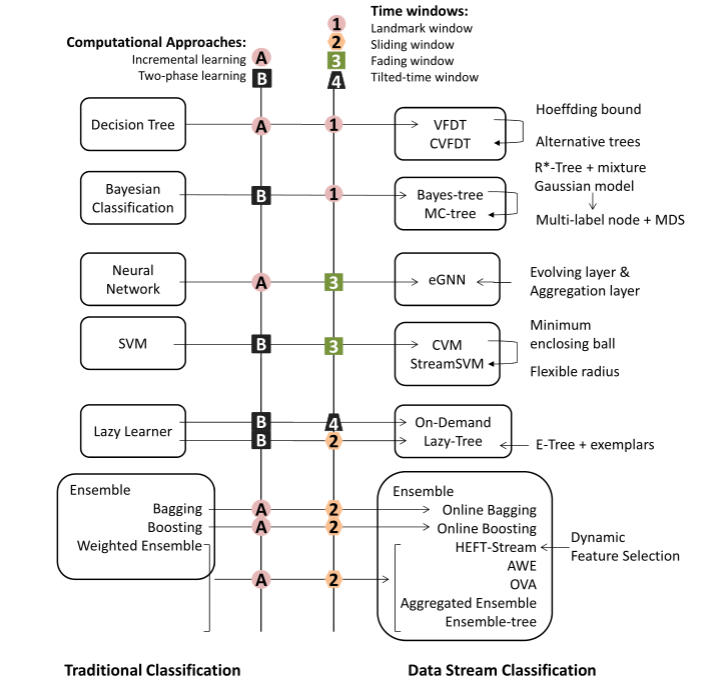
\includegraphics[width=15cm]{compare}}
\caption{مقایسه و نمایش ارتباط روش‌های سنتی یادگیری ماشین با رو‌ش‌های یادگیری در داده‌های جریانی}
\label{fig:compare}
\end{figure}

تصویر
\ref{fig:compare}
ارتباط بین روش‌های سنی رده‌بندی و رده‌بندی در داده‌های جریانی را نشان می‌دهد. رده‌بندهای سنتی در سمت چپ نوشته‌ شده‌اند و رده‌بندهای داده‌های جریانی در سمت راست. برای دسته‌بندی رده‌بندهای داده‌های جریانی به دو الگو، برای رویکرهای محساباتی و پنجره‌های زمانی نیز در وسط تصویر است.
\\
می‌توان دید که رده‌بندهای داده‌های جریانی از رده‌بندهای سنتی برگرفته شده‌اند، با این تفاوت که از رویکردهای محاسباتی مختلف و پنجره‌های زمانی متفاوتی استفاده می‌کنند. به عنوان نمونه VFDT یک گسترش از درخت‌های تصمیم برای داده‌های جریانی است. زمانی که به حد کافی داده موجود باشد، VFDT از حد هافدین برای ساختن گره‌های درخت استفاده می‌کند. در واقع این دنباله‌ای از رویکرد یادگیری افزایشی و پنجره نقطه عطفی است .CVFDT یک نسخه بهبود یافته از VFDT است که می‌تواند به وسیله‌ی ساختن درخت‌های جایگزین با رانش مفهوم سازگار شود. درخت بیز یک نسخه تغییر یافته از رده‌بندهای بیزین با دو فاز مختلف یادگیری و پنجره نقطه‌عطفی است. MCTree نیز بهبودی از درخت بیز با استفاده از گره‌های چند برچسبه است. eGNN یک شبکه عصبی است که برای کار با داده‌های جریانی طراحی شده‌است. CVM نیز نشات گرفته از رده‌بند SVM اس که از رویکرد دوفازی یادگیری و پنجره محو شونده استفاده می‌کند. StreamSVM نیز یک نسخه توسعه‌یافته CVM است که با ساختن حداقل گوی نزدیک به شکل پویا عمل می‌کند.

 
الگوریتم‌ On-Demand ، یک نسخه بهبود یافته از رده‌بندهای k-NN است که با استفاده از رویکرد یادگیری دوگامی و پنجره یک بر کار می‌کند. Lazy-Tree نیز یک نسخه بهبود‌یافته از رده‌بند k-NN است که با استفاده از رویکرد یادگیری دوگامی و و پنجره کشویی کار می‌کند.
تعداد زیادی مجمع رده‌بندها برای کار با داده‌های جریانی طراحی شده است. Bagging و Boosting آنلاین، نسخه‌های از روش‌های سنتی Bagging و Boosting با استفاده از رویکرد یادگیری افزایشی و پنجره کشویی است.


تعداد زیادی مجمع وزنی از رده‌بندها وجود دارد که از استراتژی‌های مختلف وزن‌دهی استفاده می‌کنند. برای نمونه مجمع‌های جمع‌آوری شده که از روش‌ میانگین وزنی(رای‌گیری) استفاده می‌کنند مانند HEFT-Stream ، AWE ، OVA ، Ensemble-tree که در این روش‌ها وزن متناسب با دقت رده‌بند تنظیم می‌شود. این روش‌های دنباله‌ای از رویکرد یادگیری افزایشی هستند و می‌توان فرض کرد که از پنجره کشویی استفاده می‌کنند و به طور مرسوم، اعضای رده‌بندی که دقت کمی دارند را از مجمع حذف می‌کند.

\begin{table}
  \caption{مقایسه ظرفیت‌های الگوریتم‌های مختلف یادگیری در داده‌های جریانی}
  \label{tbl:capa}
  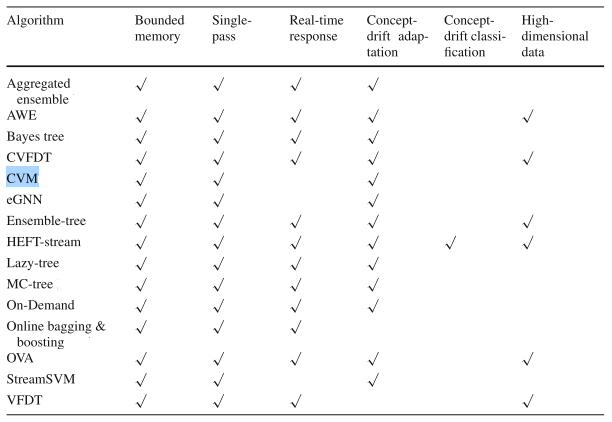
\includegraphics[width=\linewidth]{capa}
\end{table}

به طور خلاصه، در جدول
\ref{tbl:capa}
ظرفیت‌های رده‌بند های مختلف روی داده‌های جریانی، به شکل مقایسه‌ای آورده شده است. همانطور که مشهود است بسیاری از رده‌بندهای مطرح شده، عموما نمی‌توانند در آن واحد در تمام محدودیت‌های کار با داده‌های جریانی بگنجند. در این جدول در دو سطح تعامل با رانش‌ وجود دارد: این که بتوانند با رانش مفهوم سازگار شوند و این که رانش مفهوم را رده‌بندی کنند. به علاوه مشخص شده است که کدام یک از رده‌بندها می‌توانند با داده‌های با ابعاد بالا در جریان‌های داده‌ای کار می‌کند.

همانطور که دور از انتظار نیست، تمام روش‌های رده‌بندی داده‌های جریانی، یکبار داده‌ را مشاهده می‌کنند و با محدودیت حافظه مشکل چندانی ندارند. eGNN و CVM و StreamSVM نمی‌توانند بلادرنگ پاسخگو باشند و برای دادن نتیجه به زمان جهت پردازش‌هایشان احتیاج دارند. HEFT-Stream می‌تواند دو نوع رانش‌ مفهوم(هم رانش تدریجی و هم رانش ویژگی) را مشخص کند و به خوبی با آن‌ها سازگار شود. اگر درخت تصمیم به عنوان رده‌بند پایه برای روش‌های VFDT و CVFDT و AWE و OVA و درخت مجمع انتخاب شود، این روش‌ها می‌توانند با داده‌هایی با ابعاد بالا نیز کار کنند کارکنند. 


\begin{table}
  \caption{مزایا و محدودیت‌های روش‌های رده‌بندی برای داده‌های جریانی}
  \label{tbl:advant}
  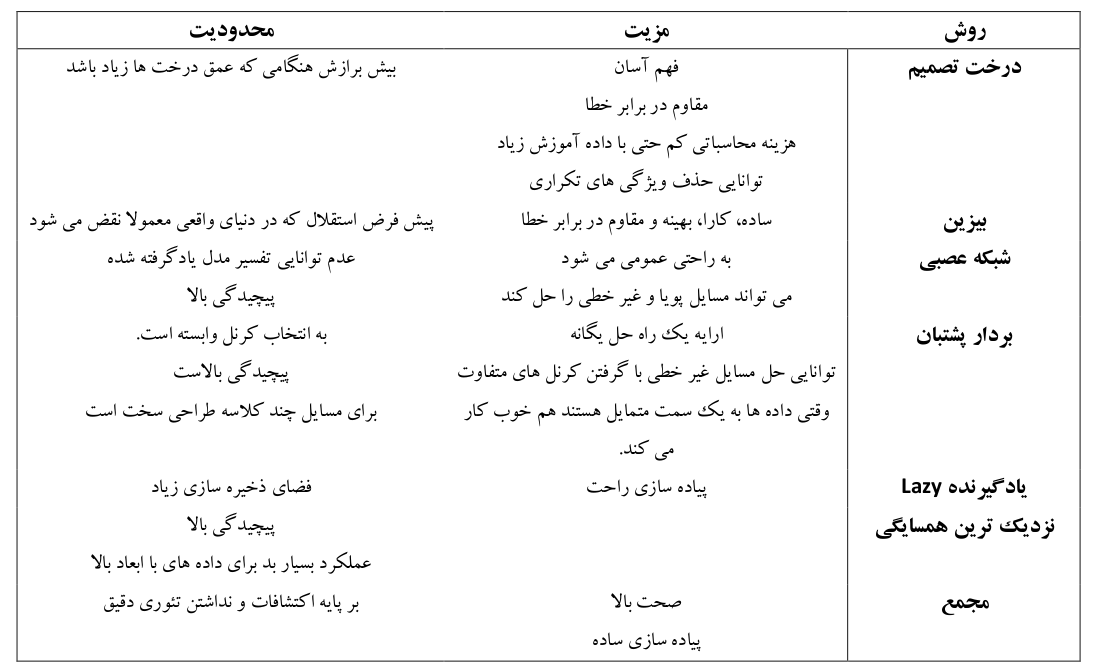
\includegraphics[width=\linewidth]{advant}
\end{table}
همانطور که دور از انتظار نیست، تمام روش‌های رده‌بندی داده‌های جریانی، یکبار داده‌ را مشاهده می‌کنند و با محدودیت حافظه مشکل چندانی ندارند. eGNN و CVM و StreamSVM نمی‌توانند بلادرنگ پاسخگو باشند و برای دادن نتیجه به زمان جهت پردازش‌هایشان احتیاج دارند. HEFT-Stream می‌تواند دو نوع رانش‌ مفهوم(هم رانش تدریجی و هم رانش ویژگی) را مشخص کند و به خوبی با آن‌ها سازگار شود. اگر درخت تصمیم به عنوان رده‌بند پایه برای روش‌های VFDT و CVFDT و AWE و OVA و درخت مجمع انتخاب شود، این روش‌ها می‌توانند با داده‌هایی با ابعاد بالا نیز کار کنند کارکنند. 

هنگامی که یک رده‌بند از رویکر محاسباتی و پنجره زمانی استفاده می‌کند بعضی مزایا و معایب که در فصل‌های قبل نیز در مورد آن‌ها بحث شد، خودشان را نشان می‌دهد. به هر روی روش‌های سنتی و رده‌بندهای داده‌های جریانی هر دو مزایا و محدودیت‌هایی دارند که در جدول
\ref{tbl:advant}
آمده است. به عنوان مثال درخت تصمیم به راحتی قابل فهم است، در برابر خطا مقاوم است، کاراست و می‌تواند خصیصه‌های تکراری را حذف کند. اما اگر عمق درخت‌ها زیاد باشد دچار مشکل بیش‌برازش
\LTRfootnote{Overfitting}
می‌شود. یادگیرنده Lazy می‌تواند به سادگی پیاده‌سازی شود اما این یادگیرنده حافظه زیادی مصرف می‌کند و در برابر داده‌هایی با ابعاد بالا مشکل دارد. مجمع‌ها صحت بالایی دارند و به سادگی پیاده‌سازی می‌شوند اما بیشترشان بر پایه اکتشافات هستند و پایه تئوری قوی ندارند.


\section{کارهای آینده در جریان‌های متنی}
از آن‌جایی که بیشتر تحقیقات در داده‌های جریانی مربوط به دهه‌ی اخیر بوده است، هنوز مسایل زیادی برای تحقیقات وجود دارد. با توجه موضوع این گزارش، در این بخش، تحقیقات آینده‌ای که مربوط به کاوش و یادگیری درباره داده‌های جریانی متنی است را مطرح می‌کنیم.

\subsection{انتخاب پویای ویژگی}

\begin{figure}%[ht]
\centerline{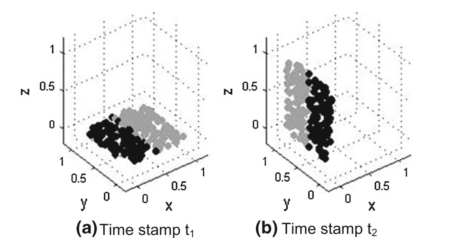
\includegraphics[width=10cm]{dynamic_feature}}
\caption{یک مثال که نشان می‌دهد چگونه ذات ویژگی‌های بااهمیت طی زمان می‌تواند تغییر کند.}
\label{fig:dynamic_feature}
\end{figure}

در همه‌ی داده‌های با ابعاد بالا، که داده‌های متنی هم جز آن‌هاست تمام ویژگی‌ها(خصیصه‌ها) در فرایند با اهمیت هستند. در واقع سه نوع مختلف ویژگی وجود داد: (یک) ویژگی‌های غیر مرتبط، (دو) ویژگی‌های مرتبط اما تکراری و (سه) ویژگی‌های مرتنبط و غیر تکراری. وظیفه‌ی اصلی موضوع انتخاب ویژگی، استخراج مجموعه‌ی ویژگی‌های مرتبط و غیرتکراری از ویژگی‌هاست که فرایند یادگیری را با معنی‌تر و سریع‌تر کند. در ادبیات موضوع، روش‌های انتخاب ویژگی به سه دسته تقسیم می‌شوند: فیلتر، پوشش
\LTRfootnote{Wrapper}
و مدل‌های نهفته
\LTRfootnote{Embedded models}
.

مدل فیلتر به عنوان یک معیار مستقل برای ارزیابی مجموعه‌ی ویژگی‌ها به‌ کار برده می‌شود، بنابراین این روش فقط به مشخصه‌های عمومی داده اتکا می‌کند. مدل پوششی، به همراه الگوریتم‌های یادگیری اجرا می‌شود از کارایی الگوریتم‌های یادگیری برای ارزیابی ویژگی‌ها استفاده می‌کند. مدل‌های ترکیبی از مزیت دو مدل گفته شده استفاده می‌کند.

اهمیت ویژگی‌ها در داده‌های جریانی تغییر می‌کند و محدود بودن یه یک بازه‌ی زمان مشخص است. ویژگی‌های که پیش‌از این باارزش فرض‌ می‌شد ممکن است نامربوط شوند و برعکس ممکن است ویژگی‌های استفاده نشده در آینده با اهمیت شوند. بنابراین استفاده از روش‌های پویای انتخاب ویژگی برای رصدکردن تغییرات ویژگی‌ها ضروری است. شکل
\ref{fig:dynamic_feature}
ذات پویای ویژگی‌های کلیدی را نشان می‌دهد. فرض کنید داده‌های ما سه ویژگی و دو کلاس داشته باشند: نقطه‌های سیاه و قهوه‌ای نمایانگر کلاس‌های مثبت و منفی هستند. در زمان $t_1 $، ویژگی‌های با ارزش x و y هستند چون داده روی صفحه xy جا گرفته است. پس از این که توزیع داده فرق می‌کند، ویژگی‌های با اهمیت y و z می‌شوند.

پس از بررسی تعداد زیادی از الگوریتم‌های یادگیری، مشاهده شد که تنها اندکی از آن‌ها می‌توانند با داده‌هایی با ابعاد بالا کار کنند و محدودیت‌های زیادی دارند. بعضی از رده‌بندهایی که با داده‌های با ابعاد بالا کار می‌کنند. این الگوریتم‌ها معمولا از درخت تصمیم به عنوان رده‌بند پایه استفاده می‌کنند و توانایی حذف ویژگی‌های تکراری را ندارند. HEFT-Stream تنها مجمع رده‌بندی است که هم ویژگی‌های نامرتبط و هم ویژگی‌های تکرای را حذف می‌کند و با هر نوع رده‌بندی کار می‌کند. HEFT-Stream از مدل فیلتر استفاده می‌کند و مستقل از نوع اعضای رده‌بند است. به هر حال مساله انتخاب پویای ویژگی یک مساله باز است که نیاز به تحقیقات بیشتری دارد.


\subsection{کاوش در جریان‌های متنی}
در سال‌های اخیر تعداد زیادی از نرم‌افزار‌های مبتنی بر وب، حجم زیادی از جریان‌های متنی را تولید می‌کنند. به عنوان مثال، اعضای شبکه‌های اجتماعی به طور مداوم با پیام‌های متنی با یکدگیر تعامل می‌کنند. بسیاری از پرتال‌ها اخبار را بر اساس علاقه‌مندی خوانندگان، بلادرنگ به آن‌ها نشان می‌دهند و خزنده‌های وب میلیون‌ها صفحه را برای نمایه سازی ذخیره می‌کنند. کاوش در جریان‌های متنی، که با سایر وظیفه‌هایی مانند فیلترکردن هرزنامه‌ها مرتبط است.

به طور عمومی، روش‌های داده‌های جریانی با ابعاد بالا می‌توانند برای داده‌های متنی استفاده شوند، البته این موضوع باید بعد از جمع‌آوری و عملیات پیش‌پردازش شامل حذف کلمات ایست، ریشه‌یابی، نگاشت به نمایش‌هایی از قبیل کیسه‌ای از کلمات
\LTRfootnote{Bag of Word}
، TF-IDF
و جداسازی عبارت‌ها باشد. اما داده‌های متنی پیچیده‌تر از داده‌های با ابعاد بالا هستند، چرا که معمولا این داده‌ها غیرساخت‌یافته، شامل خطاهای سطح بالا و در فرمت‌های گوناگون هستند. به علاوه در داده‌های متنی بیشتر تغییر موضوع در زمان رخ می‌دهد. همین باعث شده است که کاوش در جریان‌های متنی یک کار دلهره‌آور باشد.

		% فصل دوم: آشنایی مقدماتی با لاتک

% مراجع

\pagestyle{empty}
{
\onehalfspacing
\bibliographystyle{acm-fa}%{chicago-fa}%{plainnat-fa}%
\bibliography{MyReferences}
}

\pagestyle{fancy}

\appendix                           %فصلهای پس از این قسمت به عنوان ضمیمه خواهند آمد.
% اگر شما پیوست اول  خود را در فایلی به جز appendix1 همراه با این کلاس نوشته‌اید باید چندخط اول appendix1 را در فایل خود کپی کنید.
%% !TeX root=main.tex
% دستورات زیر باید در اولین فایل پیوست باشند. آنها را حذف نکنید!
\addtocontents{toc}{
    \protect\renewcommand\protect\cftchappresnum{\appendixname~}%
    \protect\setlength{\cftchapnumwidth}{\mylenapp}}%
    
\chapter{مدیریت مراجع در لاتک}\label{App:RefMan}
\thispagestyle{empty}

در بخش \ref{Sec:Ref} اشاره شد که با دستور 
 \lr{\textbackslash bibitem}
  می‌توان یک مرجع را تعریف نمود و با فرمان
 \lr{\textbackslash cite}
  به آن ارجاع داد. این روش برای تعداد مراجع زیاد و تغییرات آنها مناسب نیست. در ادامه به صورت مختصر توضیحی در خصوص برنامه \lr{BibTeX} که همراه با توزیع‌های معروف تِک عرضه می‌شود و نحوه استفاده از آن در زی‌پرشین خواهیم داشت.

\section{ مدیریت مراجع با  \texorpdfstring{\lr{Bib\TeX}}{Bib\TeX} }
یکی از روش‌های قدرتمند و انعطاف‌پذیر برای نوشتن مراجع مقالات و مدیریت مراجع در لاتک، استفاده از  \lr{BibTeX} است.
 روش کار با  \lr{BibTeX} به این صورت است که مجموعه‌ی همه‌ی مراجعی را که در \پ استفاده کرده یا خواهیم کرد، 
در پرونده‌ی جداگانه‌ای نوشته و به آن فایل در سند خودمان به صورت مناسب لینک می‌دهیم.
 کنفرانس‌ها یا مجله‌های گوناگون برای نوشتن مراجع، قالب‌ها یا قراردادهای متفاوتی دارند که به آنها استیلهای مراجع گفته می‌شود.
 در این حالت به کمک ‌استیل‌های \lr{BibTeX} خواهید توانست تنها با تغییر یک پارامتر در پرونده‌ی ورودی خود، مراجع را مطابق قالب موردنظر تنظیم کنید. 
 بیشتر مجلات و کنفرانس‌های معتبر یک پرونده‌ی سبک (\lr{BibTeX Style}) با پسوند \lr{bst} در وب‌گاه خود می‌گذارند که برای همین منظور طراحی شده است.

به جز نوشتن مقالات این سبک‌ها کمک بسیار خوبی برای تهیه‌ی مستندات علمی همچون پایان‌نامه‌هاست که فرد می‌تواند هر قسمت از کارش را که نوشت مراجع مربوطه را به بانک مراجع خود اضافه نماید. با داشتن چنین بانکی از مراجع، وی خواهد توانست به راحتی یک یا چند ارجاع به مراجع و یا یک یا چند بخش را حذف یا اضافه ‌نماید؛ 
مراجع به صورت خودکار مرتب شده و فقط مراجع ارجاع داده شده در قسمت کتاب‌نامه خواهندآمد. قالب مراجع به صورت یکدست مطابق سبک داده شده بوده و نیازی نیست که کاربر درگیر قالب‌دهی به مراجع باشد. 
در این جا مجموعه‌ سبک‌های بسته \lr{Persian-bib} که برای  زی‌پرشین آماده شده‌اند به صورت مختصر معرفی شده و روش کار با آن‌ها گفته می‌شود. برای اطلاع بیشتر به راهنمای بسته‌ی \lr{Persian-bib} مراجعه فرمایید.
\subsection{سبک‌های فعلی قابل استفاده در زی‌پرشین}
در حال حاضر فایلهای سبک زیر برای استفاده در زی‌پرشین آماده شده‌اند:

\singlespacing
\begin{description}
\item [unsrt-fa.bst] این سبک متناظر با \lr{unsrt.bst} می‌باشد. مراجع به ترتیب ارجاع در متن ظاهر می‌شوند.
\item [plain-fa.bst] این سبک متناظر با \lr{plain.bst} می‌باشد. مراجع بر اساس نام‌خانوادگی نویسندگان، به ترتیب صعودی مرتب می‌شوند.
 همچنین ابتدا مراجع فارسی و سپس مراجع انگلیسی خواهند آمد.
\item [acm-fa.bst] این سبک متناظر با \lr{acm.bst} می‌باشد. شبیه \lr{plain-fa.bst} است.  قالب مراجع کمی متفاوت است. اسامی نویسندگان انگلیسی با حروف بزرگ انگلیسی نمایش داده می‌شوند. (مراجع مرتب می‌شوند)
\item [ieeetr-fa.bst] این سبک متناظر با \lr{ieeetr.bst} می‌باشد. (مراجع مرتب نمی‌شوند)
\item [plainnat-fa.bst] این سبک متناظر با \lr{plainnat.bst} می‌باشد. نیاز به بستهٔ \lr{natbib} دارد. (مراجع مرتب می‌شوند)
\item [chicago-fa.bst] این سبک متناظر با \lr{chicago.bst} می‌باشد. نیاز به بستهٔ \lr{natbib} دارد. (مراجع مرتب می‌شوند)
\item [asa-fa.bst] این سبک متناظر با \lr{asa.bst} می‌باشد. نیاز به بستهٔ \lr{natbib} دارد. (مراجع مرتب می‌شوند)
\end{description}
\doublespacing

با استفاده از استیلهای فوق می‌توانید به انواع مختلفی از مراجع فارسی و لاتین ارجاع دهید. به عنوان نمونه مرجع 
\cite{Omidali82phdThesis}
 یک نمونه پروژه دکترا (به فارسی) و مرجع 
\cite{Vahedi87} یک نمونه مقاله مجله فارسی است.
مرجع 
\cite{Amintoosi87afzayesh}  یک نمونه  مقاله کنفرانس فارسی و
مرجع 
\cite{Pedram80osool} یک نمونه کتاب فارسی با ذکر مترجمان و ویراستاران فارسی است. مرجع 
\cite{Khalighi07MscThesis} یک نمونه پروژه کارشناسی ارشد انگلیسی و
\cite{Khalighi87xepersian} هم یک نمونه متفرقه  می‌باشند.

مراجع 
\cite{Gonzalez02book,Baker02limits} 
نمونه کتاب و مقاله انگلیسی هستند.
استیل مورد استفاده در این \پ \lr{acm-fa} است که خروجی آنرا در بخش مراجع می‌توانید مشاهده کنید.
نمونه  خروجی سبک \lr{asa-fa} در شکل \ref{fig:asafa} آمده است.

\begin{figure}[t]
\centering
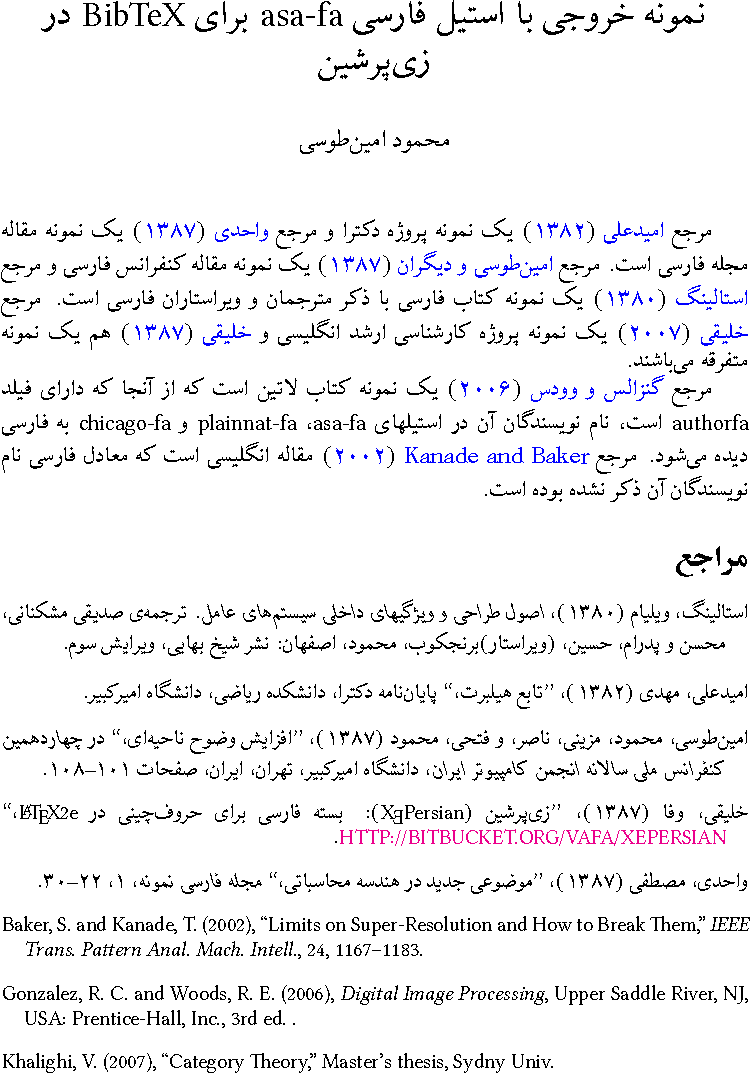
\includegraphics[width=.8\textwidth]{asa-fa-crop.pdf}
\caption{نمونه خروجی با سبک \lr{asa-fa}}
\label{fig:asafa}
\end{figure} 

\subsection{ نحوه استفاده از سبک‌های فارسی}


برای استفاده از بیب‌تک باید مراجع خود را در یک فایل با پسوند \lr{bib} ذخیره نمایید. یک فایل \lr{bib} در واقع یک پایگاه داده از مراجع\LTRfootnote{Bibliography Database}  شماست که هر مرجع در آن به عنوان یک رکورد از این پایگاه داده
با قالبی خاص ذخیره می‌شود. به هر رکورد یک مدخل\LTRfootnote{Entry} گفته می‌شود. یک نمونه مدخل برای معرفی کتاب \lr{Digital Image Processing} در ادامه آمده است:

\singlespacing
\begin{LTR}
\begin{verbatim}
@BOOK{Gonzalez02image,
  AUTHOR =      {Rafael Gonzalez and Richard Woods},
  TITLE =       {Digital Image Processing},
  PUBLISHER =   {Prentice-Hall, Inc.},
  YEAR =        {2006},
  EDITION =     {3rd},
  ADDRESS =     {Upper Saddle River, NJ, USA}
}
\end{verbatim}
\end{LTR}
\doublespacing

در مثال فوق، \lr{@BOOK} مشخصه‌ی شروع یک مدخل مربوط به یک کتاب و \lr{Gonzalez02book} برچسبی است که به این مرجع منتسب شده است.
 این برچسب بایستی یکتا باشد. برای آنکه فرد به راحتی بتواند برچسب مراجع خود را به خاطر بسپارد و حتی‌الامکان برچسب‌ها متفاوت با هم باشند معمولاً از قوانین خاصی به این منظور استفاده می‌شود. یک قانون می‌تواند فامیل نویسنده‌ی اول+دورقم سال نشر+اولین کلمه‌ی عنوان اثر باشد. به \lr{AUTHOR} و $\dots$ و \lr{ADDRESS} فیلدهای این مدخل گفته می‌شود؛ که هر یک با مقادیر مربوط به مرجع مقدار گرفته‌اند. ترتیب فیلدها مهم نیست. 

انواع متنوعی از مدخل‌ها برای اقسام مختلف مراجع همچون کتاب، مقاله‌ی کنفرانس و مقاله‌ی ژورنال وجود دارد که برخی فیلدهای آنها با هم متفاوت است. 
نام فیلدها بیانگر نوع اطلاعات آن می‌باشد. مثالهای ذکر شده در فایل \lr{MyReferences.bib} کمک خوبی به شما خواهد بود. 
%این فایل یک فایل متنی بوده و با ویرایشگرهای معمول همچون \lr{Notepad++} قابل ویرایش می‌باشد. برنامه‌هایی همچون 
%\lr{TeXMaker}
% امکاناتی برای نوشتن این مدخل‌ها دارند و به صورت خودکار فیلدهای مربوطه را در فایل \lr{bib}  شما قرار می‌دهند.  
با استفاده از سبک‌های فارسی آماده شده، محتویات هر فیلد می‌تواند به فارسی نوشته شود، ترتیب مراجع و نحوه‌ی چینش فیلدهای هر مرجع را سبک مورد استفاده  مشخص خواهد کرد.

نکته: بدون اعمال تنظیمات موردنیاز \lr{Bib\TeX} در \lr{TeXWorks}، مراجع فارسی در استیل‌هایی که مراجع را به صورت مرتب شده چاپ می‌کنند، ترتیب کاملاً درستی نخواهند داشت. برای توضیحات بیشتر \cite{persianbib87userguide} را ببینید یا به سایت پارسی‌لاتک مراجعه فرمایید. تنظیمات موردنیاز در \lr{TeXMaker} اصلاح شده اعمال شده‌اند.

\textbf{برای درج مراجع خود لازم نیست نگران موارد فوق باشید. در فایل 
\lr{MyReferences.bib}
 که همراه با این \پ هست، موارد مختلفی درج شده است و کافیست مراجع خود را جایگزین موارد مندرج در آن نمایید.
}

پس از قرار دادن مراجع خود، یک بار \lr{XeLaTeX} را روی سند خود اجرا نمایید، سپس \lr{bibtex} و پس از آن دوبار \lr{XeLaTeX} را. در \lr{TeXMaker} کلید \lr{F11} و در \lr{TeXWorks} هم گزینه‌ی \lr{BibTeX} از منوی \lr{Typeset}، \lr{BibTeX} را روی سند شما اجرا می‌کنند.

برای بسیاری از مقالات لاتین حتی لازم نیست که مدخل مربوط به آنرا خودتان بنویسید. با جستجوی نام مقاله + کلمه \lr{bibtex}  در اینترنت سایتهای بسیاری همچون \lr{ACM} و \lr{ScienceDirect} را خواهید یافت که مدخل \lr{bibtex} مربوط به مقاله شما را دارند و کافیست آنرا به انتهای فایل \lr{MyReferences} اضافه کنید.

از هر یک از سبکهای \lr{Persian-bib} می‌توانید استفاده کنید، البته اگر از سه استیل آخر استفاده می‌کنید و مایلید که مراجع شما شماره بخورند باید بسته \lr{natbib} را با گزینه \lr{numbers} فراخوانی نمایید.
		% پیوست اول: مدیریت مراجع در لاتک
%% !TeX root=main.tex

\chapter{‌جدول، نمودار و الگوریتم در لاتک}\label{App:Latex:More}
\thispagestyle{empty}

در این بخش نمونه مثالهایی از جدول، نمودار و الگوریتم در لاتک را خواهیم دید.
\section{مدلهای حرکت دوبعدی}
بسیاری از اوقات حرکت بین دو تصویر از یک صحنه با یکی از مدلهای پارامتری ذکر شده در جدول \eqref{tab:MotionModels} قابل مدل نمودن می‌باشد.  
\begin{table}[ht]
\caption{مدلهای تبدیل.}
\label{tab:MotionModels}
\centering
\onehalfspacing
\begin{tabular}{|r|c|l|r|}
\hline نام مدل & درجه آزادی & تبدیل مختصات & توضیح \\ 
\hline انتقالی & ۲ & $\begin{aligned} x'=x+t_x \\ y'=y+t_y \end{aligned}$  &  انتقال دوبعدی\\ 
\hline اقلیدسی & ۳ & $\begin{aligned} x'=xcos\theta - ysin\theta+t_x \\ y'=xsin\theta+ycos\theta+t_y \end{aligned}$  &  انتقالی+دوران \\ 
\hline مشابهت & ۴ & $\begin{aligned} x'=sxcos\theta - sysin\theta+t_x \\ y'=sxsin\theta+sycos\theta+t_y  \end{aligned}$  & اقلیدسی+تغییرمقیاس \\ 
\hline آفین & ۶ & $\begin{aligned} x'=a_{11}x+a_{12}y+t_x \\ y'=a_{21}x+a_{22}y+t_y \end{aligned}$  & مشابهت+اریب‌شدگی \\ 
\hline  پروجکتیو & ۸ & $\begin{aligned} x'&=(m_1x+m_2y+m_3)/D \\ y'&=(m_4x+m_5y+m_6)/D \\ D&=m_7x+m_8y+1 \end{aligned}$  & آفین+\lr{keystone+chirping} \\ 
\hline  شارنوری & $\infty $ & $\begin{aligned} x'=x+v_x(x,y) \\ y'=y+v_y(x,y) \end{aligned}$  &  حرکت آزاد\\ 
\hline 
\end{tabular} 
\end{table}

\section{ماتریس}

شناخته‌شده‌ترین روش تخمین ماتریس هوموگرافی الگوریتم تبدیل خطی مستقیم (\lr{DLT\LTRfootnote{Direct Linear Transform}}) است.  فرض کنید چهار زوج نقطهٔ متناظر در دو تصویر در دست هستند،  $\mathbf{x}_i\leftrightarrow\mathbf{x}'_i$   و تبدیل با رابطهٔ
  $\mathbf{x}'_i = H\mathbf{x}_i$
  نشان داده می‌شود که در آن:
\[\mathbf{x}'_i=(x'_i,y'_i,w'_i)^\top  \]
و
\[ H=\left[
\begin{array}{ccc}
h_1 & h_2 & h_3 \\ 
h_4 & h_5 & h_6 \\ 
h_7 & h_8 & h_9
\end{array} 
\right]\]
رابطه زیر را برای الگوریتم  \eqref{alg:DLT} لازم دارم.
\begin{equation}\label{eq:DLT_Ah}
\left[
\begin{array}{ccc}
0^\top & -w'_i\mathbf{x}_i^\top & y'_i\mathbf{x}_i^\top \\ 
w'_i\mathbf{x}_i & 0^\top & -x'_i\mathbf{x}_i^\top \\ 
- y'_i\mathbf{x}_i^\top & x'_i\mathbf{x}_i^\top & 0^\top
\end{array} 
\right]
\left(
\begin{array}{c}
\mathbf{h}^1 \\ 
\mathbf{h}^2 \\ 
\mathbf{h}^3
\end{array} 
\right)=0
\end{equation}

\section{الگوریتم با دستورات فارسی}
با مفروضات فوق، الگوریتم \lr{DLT} به صورت نشان داده شده در الگوریتم \eqref{alg:DLT}  خواهد بود.
\begin{algorithm}[t]
\onehalfspacing
\caption{الگوریتم \lr{DLT} برای تخمین ماتریس هوموگرافی.} \label{alg:DLT}
\begin{algorithmic}[1]
\REQUIRE $n\geq4$ زوج نقطهٔ متناظر در دو تصویر 
${\mathbf{x}_i\leftrightarrow\mathbf{x}'_i}$،\\
\ENSURE ماتریس هوموگرافی $H$ به نحوی‌که: 
$\mathbf{x}'_i = H \mathbf{x}_i$.
  \STATE برای هر زوج نقطهٔ متناظر
$\mathbf{x}_i\leftrightarrow\mathbf{x}'_i$ 
ماتریس $\mathbf{A}_i$ را با استفاده از رابطهٔ \ref{eq:DLT_Ah} محاسبه کنید.
  \STATE ماتریس‌های ۹ ستونی  $\mathbf{A}_i$ را در قالب یک ماتریس $\mathbf{A}$ ۹ ستونی ترکیب کنید. 
  \STATE تجزیهٔ مقادیر منفرد \lr{(SVD)}  ماتریس $\mathbf{A}$ را بدست آورید. بردار واحد متناظر با کمترین مقدار منفرد جواب $\mathbf{h}$ خواهد بود.
  \STATE  ماتریس هوموگرافی $H$ با تغییر شکل $\mathbf{h}$ حاصل خواهد شد.
\end{algorithmic}
\end{algorithm}

\section{الگوریتم با دستورات لاتین}
الگوریتم \ref{alg:RANSAC} یک الگوریتم با دستورات لاتین است.

\begin{algorithm}[t]
\onehalfspacing
\caption{الگوریتم \lr{RANSAC} برای تخمین ماتریس هوموگرافی.} \label{alg:RANSAC}
\begin{latin}
\begin{algorithmic}[1]
\REQUIRE $n\geq4$ putative correspondences, number of estimations, $N$, distance threshold $T_{dist}$.\\
\ENSURE Set of inliers and Homography matrix $H$.
\FOR{$k = 1$ to $N$}
  \STATE Randomly choose 4 correspondence,
  \STATE Check whether these points are colinear, if so, redo the above step
  \STATE Compute the homography $H_{curr}$ by DLT algorithm from the 4 points pairs,
  \STATE $\ldots$ % الگوریتم کامل نیست
  \ENDFOR
  \STATE Refinement: re-estimate H from all the inliers using the DLT algorithm.
\end{algorithmic}
\end{latin}
\end{algorithm}

\section{نمودار}
لاتک بسته‌هایی با قابلیت‌های زیاد برای رسم انواع مختلف نمودارها دارد. مانند بسته‌های \lr{Tikz} و  \lr{PSTricks}. توضیح اینها فراتر از این پیوست کوچک است. مثالهایی از رسم نمودار را در مجموعه پارسی‌لاتک خواهید یافت. توصیه می‌کنم که حتماً مثالهایی از برخی از آنها را ببینید. راهنمای همه آنها در تک‌لایو هست. نمونه مثالهایی از بسته \lr{Tikz} را می‌توانید در \url{http://www.texample.net/tikz/examples/} ببینید.

\section{تصویر}
نمونه تصاویری در بخش قبل دیدیم. دو تصویر شیر کنار هم را هم در شکل \ref{fig:twolion} مشاهده می‌کنید.
\begin{figure}[t]
\centering 
\subfigure[شیر ۱]{ \label{fig:twolion:one}

\includegraphics[width=.3\textwidth]{lion}}
%\hspace{2mm}
\subfigure[شیر ۲]{ \label{fig:twolion:two}

\includegraphics[width=.3\textwidth]{lion}}
\caption{دو شیر}
\label{fig:twolion} %% label for entire figure
\end{figure}

%\baselineskip=.75cm
\onehalfspacing
%\chapter*{واژه‌نامه فارسی به انگلیسی}\markboth{واژه‌نامه فارسی به انگلیسی}{واژه‌نامه فارسی به انگلیسی}
\addcontentsline{toc}{chapter}{واژه‌نامه فارسی به انگلیسی}
\thispagestyle{empty}

\englishgloss{Probabilistic}{احتمالی}
\englishgloss{Valuation}{ارزیابی}
\englishgloss{Measure}{اندازه }
\englishgloss{Stably}{پایدار}
\englishgloss{Weak Topology}{توپولوژی ضعیف}
\englishgloss{Powerdomain}{دامنه‌توانی}
\englishgloss{Function Space}{فضای تابع}
\englishgloss{Semantic Domain}{دامنه معنایی}
\englishgloss{Program Fragment}{قطعه‌برنامه}
\englishgloss{Dcpo}{مجموعه جزئاً مرتب کامل جهت‌دار}
\englishgloss{Ordered}{مرتب}
%\chapter*{واژه‌نامه  انگلیسی به  فارسی}\markboth{واژه‌نامه  انگلیسی به  فارسی}{واژه‌نامه  انگلیسی به  فارسی}
\addcontentsline{toc}{chapter}{واژه‌نامه  انگلیسی به  فارسی}
\thispagestyle{empty}

\persiangloss{مجموعه جزئاً مرتب کامل جهت‌دار}{Dcpo}
\persiangloss{فضای تابع}{Function Space}
\persiangloss{اندازه }{Measure}
\persiangloss{مرتب}{Ordered}
\persiangloss{دامنه‌توانی}{Powerdomain}
\persiangloss{احتمالی}{Probabilistic}
\persiangloss{قطعه‌برنامه}{Program Fragment}
\persiangloss{دامنه معنایی}{Semantic Domain}
\persiangloss{پایدار}{Stably}
\persiangloss{ارزیابی}{Valuation}
\persiangloss{توپولوژی ضعیف}{Weak Topology}

\printindex
%% !TeX root=main.tex
% در این فایل، عنوان پایان‌نامه، مشخصات خود و چکیده پایان‌نامه را به انگلیسی، وارد کنید.

%%%%%%%%%%%%%%%%%%%%%%%%%%%%%%%%%%%%
\baselineskip=.6cm
\begin{latin}
\latinuniversity{Iran University of Science and Technology}
\latinfaculty{Computer Engineering Department}
\latinsubject{Computer Engineering }
\latinfield{Artificial Intelligence}
\latintitle{‫‪A‬‬ ‫‪Survey‬‬ ‫‪on‬‬ ‫‪Learning‬‬ ‫‪Algorithms‬‬ ‫‪for‬‬ ‫‪Text‬‬ ‫‪Streams‬‬}
\firstlatinsupervisor{Dr. Behroz Minaei Bidgoli}
%\secondlatinsupervisor{Second Supervisor}
%\firstlatinadvisor{First Advisor}
%\secondlatinadvisor{Second Advisor}
\latinname{Vahid}
\latinsurname{Kharazi}
\latinthesisdate{Octobr 2016}
\latinkeywords{Machine Learning, Data Stream, Text Mining, Text Proccessing}
%\en-abstract{
%This thesis studies on writing projects, theses and dissertations using IUST-Thesis Class. It ...
%}
\latinfirstPage
\end{latin}

\label{LastPage}

\end{document}